\chapter{Software}
The \ind{SensorBoard} hardware has two programmable CPUs and several configurable chips. The main \ind{ESP32} CPU (two low-power Xtensa 32-bit LX6 microprocessors) \cite{espressif:ESP-WROOM-32} is programmable via USB or Bluetooth or \ac{JTAG}. The \ac{JTAG} connector is not present on the \ind{SensorBoard}. The second microcontroller is a part of BMF055 \cite{bosch:BMF055} multifunctional chip. It is Atmel SAMD20 \cite{atmel:samd20} with ARM Cortex-M0+ CPU programmable via \ac{SWD} interface \cite{SWDinterface}.

\paragraph{Microcontrollers:}
\begin{enumerate}
    \item Espressif ESP-WROOM-32 \cite{espressif:ESP-WROOM-32}:
    \begin{itemize}
        \item dual core, 240 MHz, 448 kB ROM, 520 kB SRAM, 4 MB SPI flash memory
        \item Designated for main program handling all communication and interaction with user or other devices.
    \end{itemize}
    \item Atmel SAMD20 \cite{atmel:samd20}:
    \begin{itemize}
        \item ARM Cortex-M0+ CPU, 48 MHz, 32 kB SRAM, 256 kB flash memory
        \item Designated for processing inertial data (for example computing \ind{sensor fusion}), it can be used for example as an emulator of other sensors or as a simple flight controller.
    \end{itemize}
\end{enumerate}

\begin{figure}
    \centering
    \caption{Schema of available modules inside the SensorBoard hardware}
    \label{fig:SWmodules}
    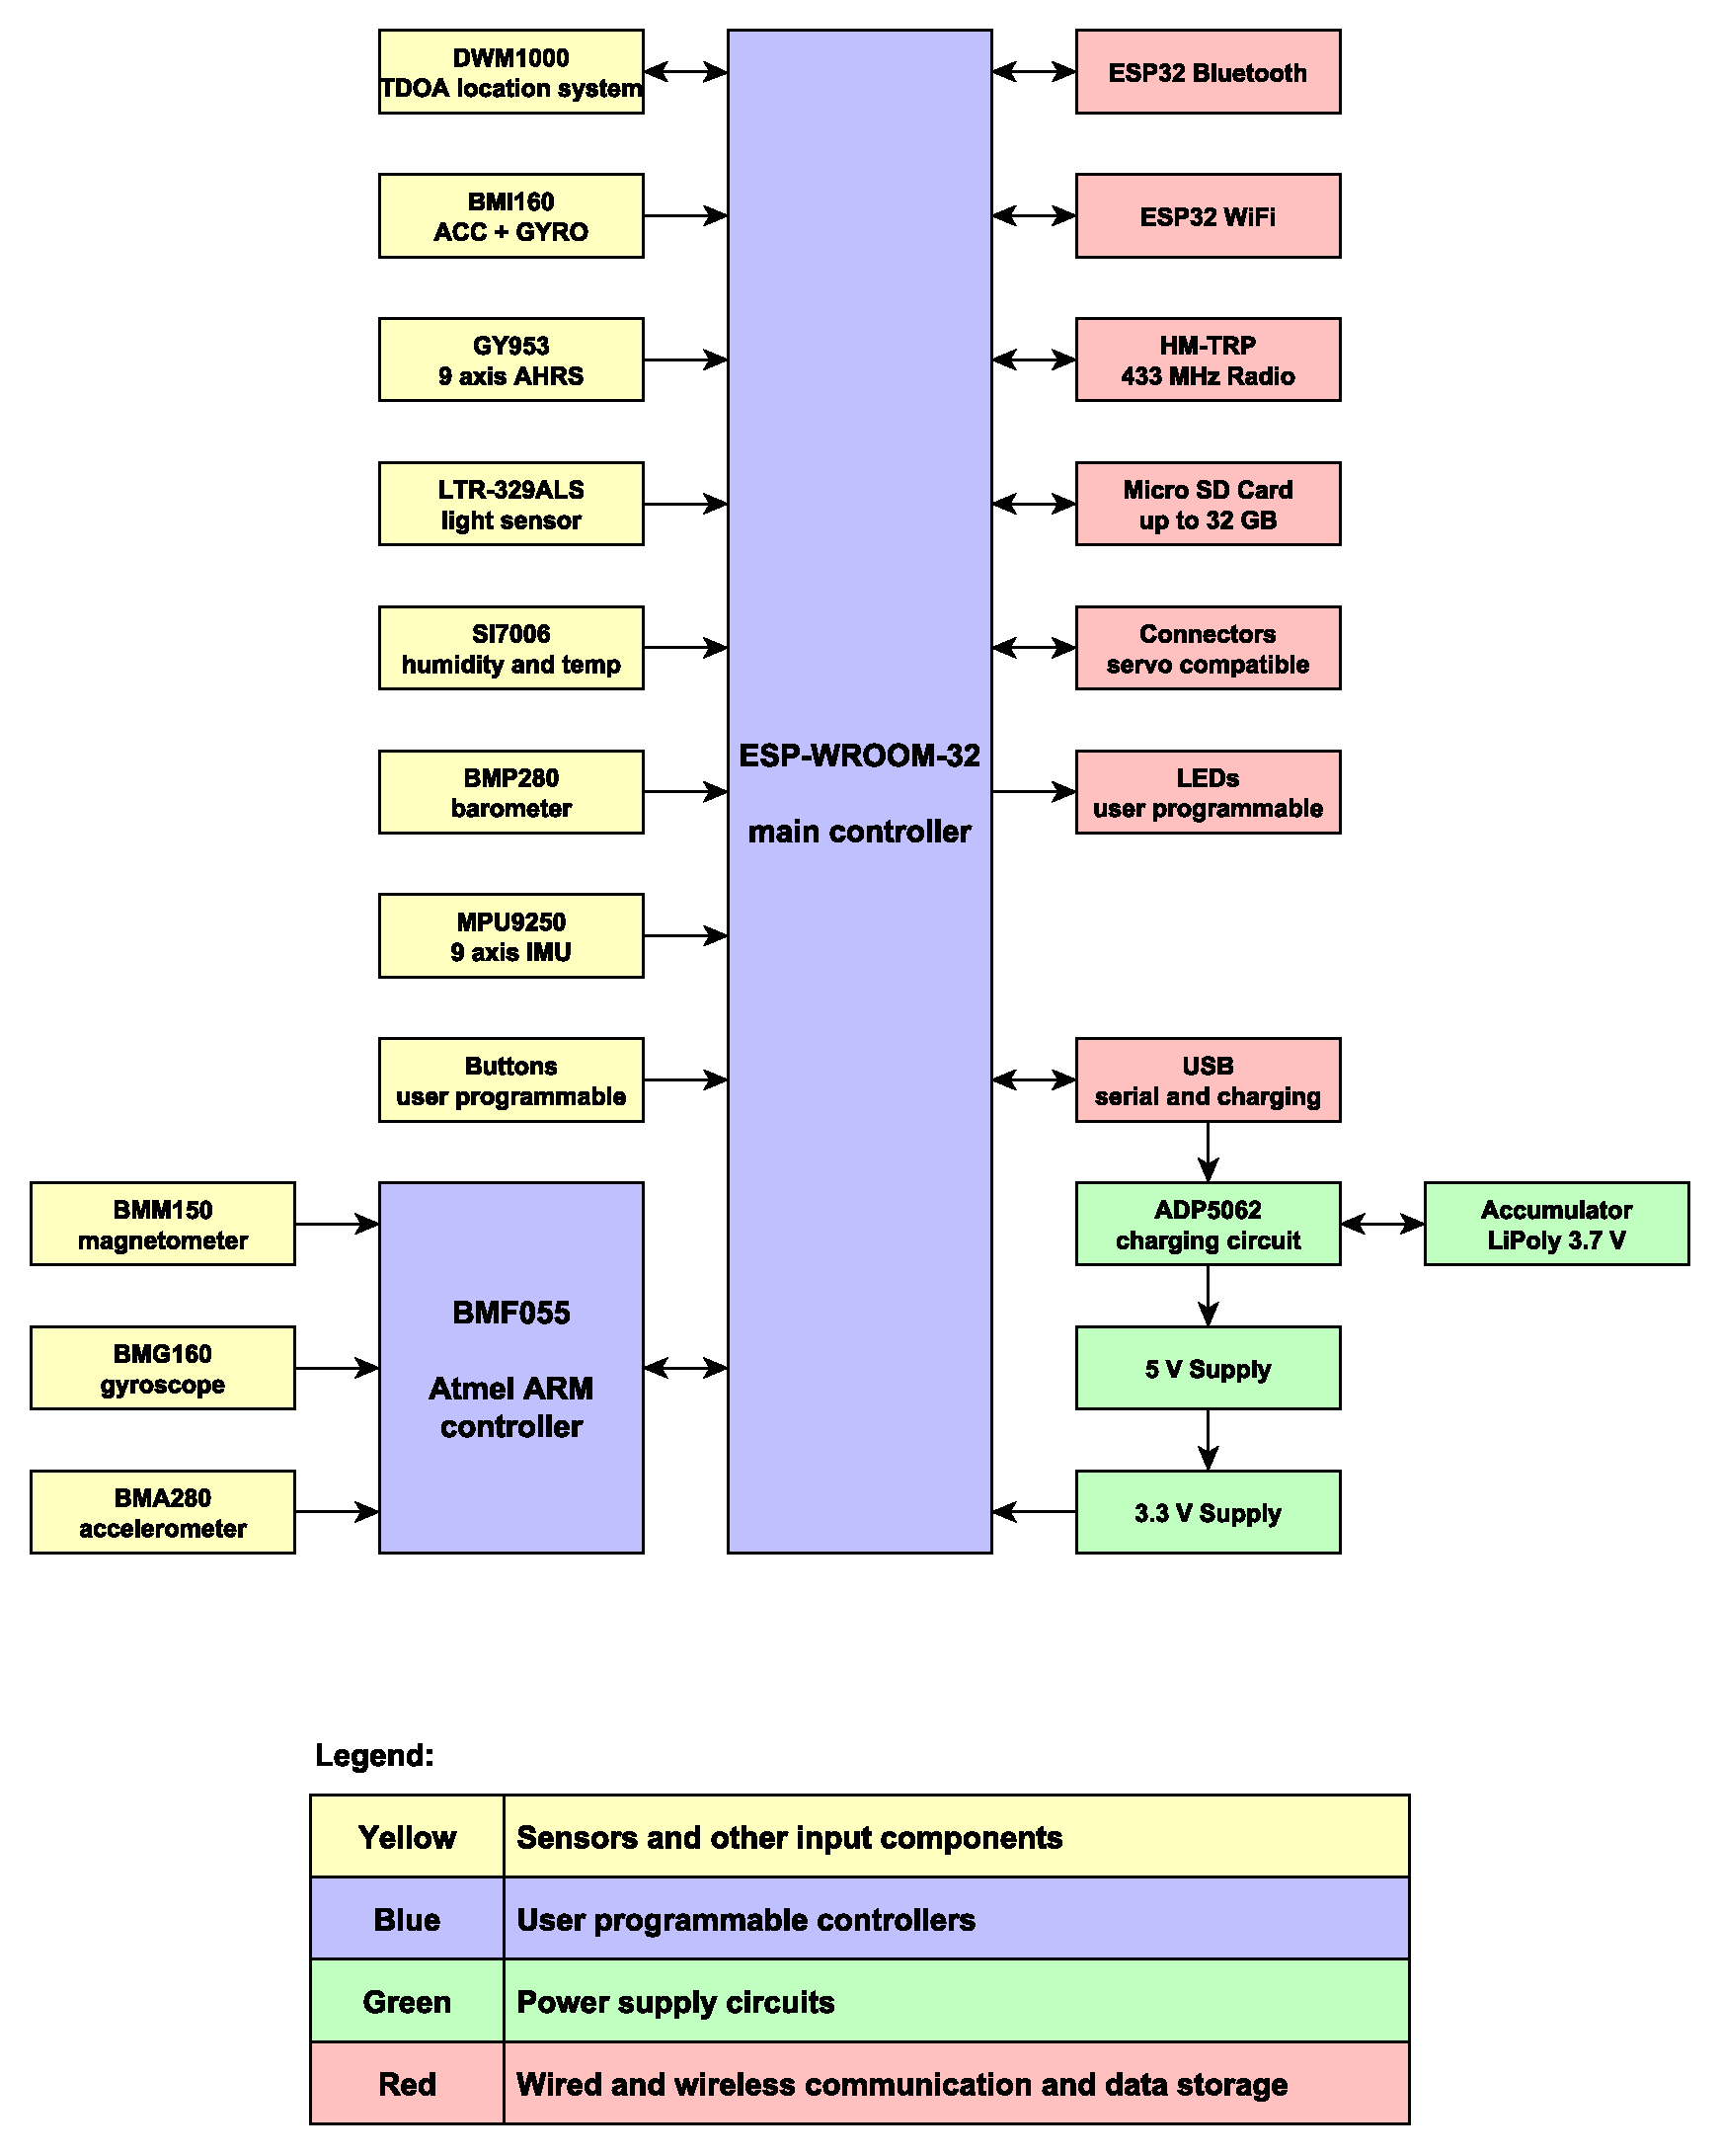
\includegraphics[width=\linewidth]{img/SensorBoardSchema.pdf}
\end{figure}

\section{Programming the Board}
Each processor on the \ind{SensorBoard} has to be programmed separately via its interface. Only \ind{ESP32} \cite{espressif:ESP-WROOM-32} (main processor) can be programmed over the air via Bluetooth. This feature is disabled by default. The pinout and other information about the \ind{SensorBoard} and BMF055 board are described in appendix \ref{hardwareDocumentation}.

\subsection{Programming ESP32}
There are several ways how to program and use the \ind{ESP32} \cite{espressif:ESP-WROOM-32} controller. The official framework is \ac{ESP-IDF} \cite{espressif:ESP-IDF} and supports all the chip functionality. The \ac{ESP-IDF} framework is \ac{POSIX} compatible.

The chip can be programmed using Arduino compatible framework \cite{espressif:ArduinoCore} which creates an easy way for prototyping and learning, but does not offer all the functionality of the chip. The Arduino framework uses the \ac{ESP-IDF} framework, so we can create "hybrid" programs that use both frameworks.

The last mentioned programming method is scripting in Python. We can upload the \ind{MicroPython} \cite{MicroPython} firmware directly to the \ind{ESP32} controller. The Python libraries, scripts and other files are stored on the SD card. The MicroPython firmware supports most of the hardware functionality, but there are still some restrictions.

Although, there are some other ways how to create a program for this hardware, many of them use one of the mentioned frameworks. For example, we can create a program in Simulink and then export the code to the \ind{ESP32} controller. \cite{ArduinoSimulink}

\subsubsection{ESP-IDF Framework}
The \ac{ESP-IDF} framework is almost \ac{POSIX} compatible. \cite{ESP32posix} It supports many \ac{POSIX} compatible functions, but it still does not support all of them. It means that we can compile many \ac{POSIX} compatible programs for \ind{ESP32}, but not all of them.

We can follow the official \ind{ESP32} programming guide \cite{ESP32programmingGuide} to set up the environment and program the board. The user can do everything from the terminal (command line). The figure \ref{ESP32menuconfig} shows a configuration tool used for setup the program before the first compilation and upload to the \ind{ESP32} microcontroller.

\begin{figure}
    \centering
    \caption{Configuration of the ESP-IDF program in terminal before the first compilation}
    \label{ESP32menuconfig}
    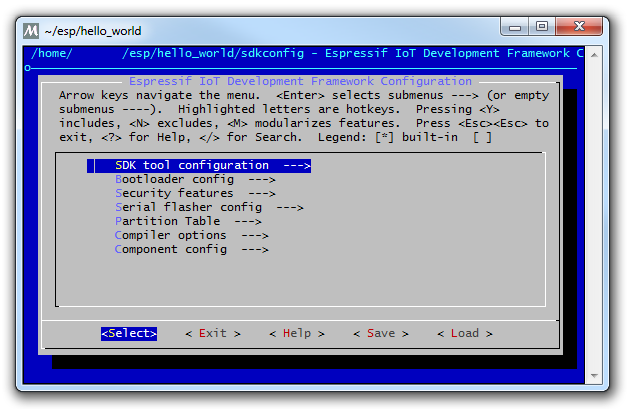
\includegraphics[width=\linewidth]{img/ESP32menuconfig.png}
\end{figure}

If we prefer some GUI for development of our software we have several options. I will mention two of them:
\begin{enumerate}
    \item \textbf{Eclipse IDE} can be setup using the guide in \ac{ESP-IDF} Programming Guide \cite{ESP32eclipse}. In my opinion, the compilation of our programs is very slow when we use this option. The figure \ref{ESP32eclipse} shows the \ind{SensorBoard} project opened in Eclipse IDE.
    \item \textbf{PlatformIO IDE} is an open source ecosystem for \ac{IoT} development. \cite{PlatformIO} There is integrated \ac{ESP-IDF} and Arduino framework for \ind{ESP32} microcontrollers. This option was more familiar to me with much faster compilation process. I have used the PlatformIO ecosystem inside Atom \cite{AtomEditor} advanced text editor. The figure \ref{ESP32atom} shows the \ind{SensorBoard} project opened in Atom editor with PlatformIO plugin.
\end{enumerate}

\begin{figure}
    \centering
    \caption{The SensorBoard project opened in Eclipse IDE}
    \label{ESP32eclipse}
    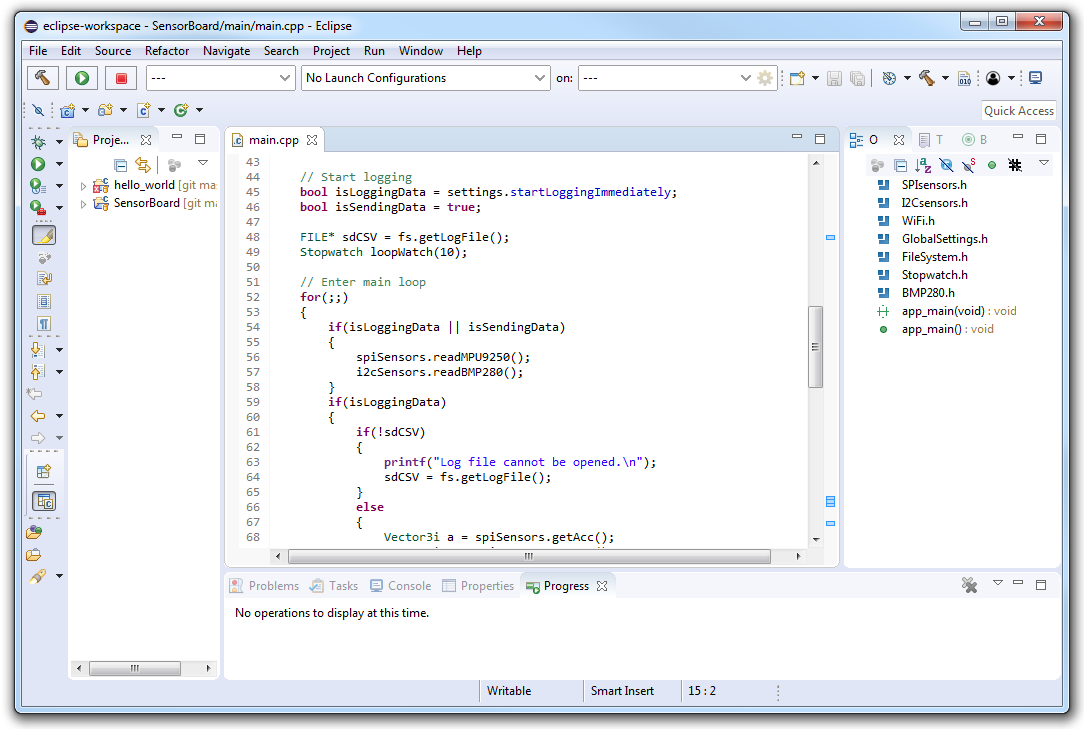
\includegraphics[width=\linewidth]{img/ESP32eclipse.png}
\end{figure}

\begin{figure}
    \centering
    \caption{The SensorBoard project opened in Atom text editor with PlatformIO plugin}
    \label{ESP32atom}
    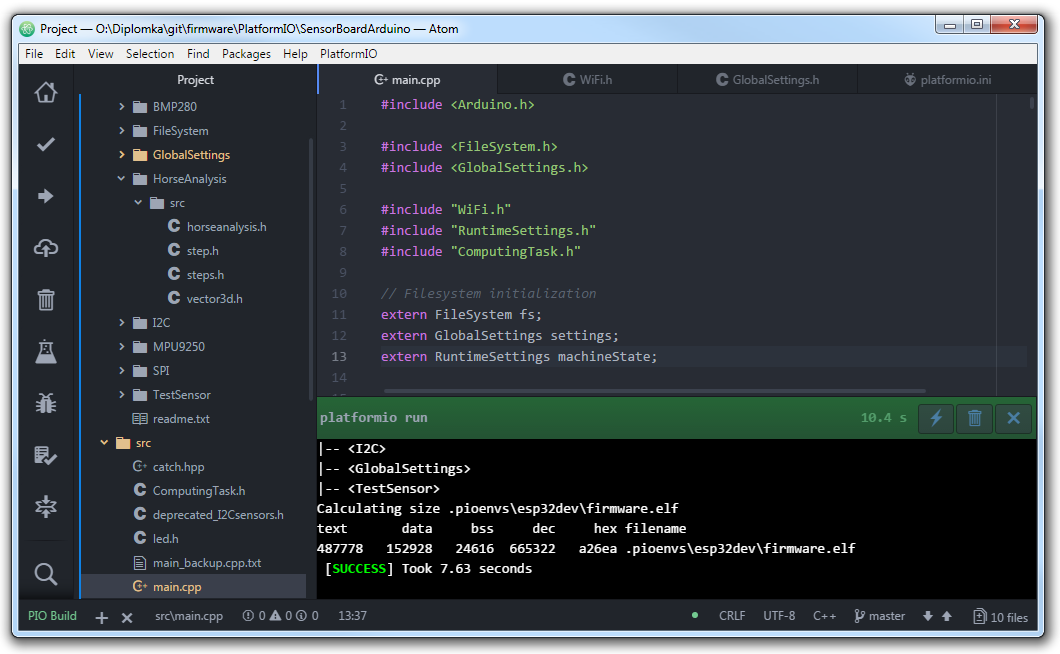
\includegraphics[width=\linewidth]{img/ESP32atom.png}
\end{figure}

\subsubsection{Arduino Compatibility}
The Arduino compatible framework for \ind{ESP32} \cite{espressif:ArduinoCore} is dependent on \ac{ESP-IDF} framework \cite{espressif:ESP-IDF}. It means that we can use both -- the \ac{ESP-IDF} functions and the Arduino functions -- in our programs. The Arduino framework is primarily targeted for beginners and for fast prototyping. I do not recommend to use this framework for advanced applications, because it does not cover the whole \ind{ESP32} functionality. We can develop our Arduino compatible programs in Arduino IDE, but we can use the PlatformIO ecosystem, too. It means that we can use the same environment like in the figure \ref{ESP32atom}. All libraries are downloaded and installed automatically inside the PlatformIO. We have to set only the \texttt{platformio.ini} file in the root directory of our project. We can add a line \texttt{framework = arduino} for Arduino compatible programs and a line \texttt{framework = espidf} for programs using the \ac{ESP-IDF} framework.

\subsubsection{MicroPython Compatibility}
The built MicroPython binary for \ind{ESP32} can be directly downloaded from MicroPython website. \cite{MicroPython} We can directly flash this binary to our \ind{ESP32} controller (to the \ind{SensorBoard}) and then directly run our Python scripts. Of course, it is possible to download the MicroPython source code from the same website. The MicroPython allows to control the \ind{SensorBoard} via Python serial terminal, so we can send a separate command via this serial terminal or run the whole Python scripts stored as files in the SD card. The SD card slot is a part of the \ind{SensorBoard}. One of the Python scripts on the SD card can be configured to be executed automatically after powering on the \ind{SensorBoard}. The running Python serial terminal on the \ind{SensorBoard} is shown in figure \ref{ESP32PythonLorris}.

\begin{figure}
    \centering
    \caption{The running Python serial terminal on the SensorBoard}
    \label{ESP32PythonLorris}
    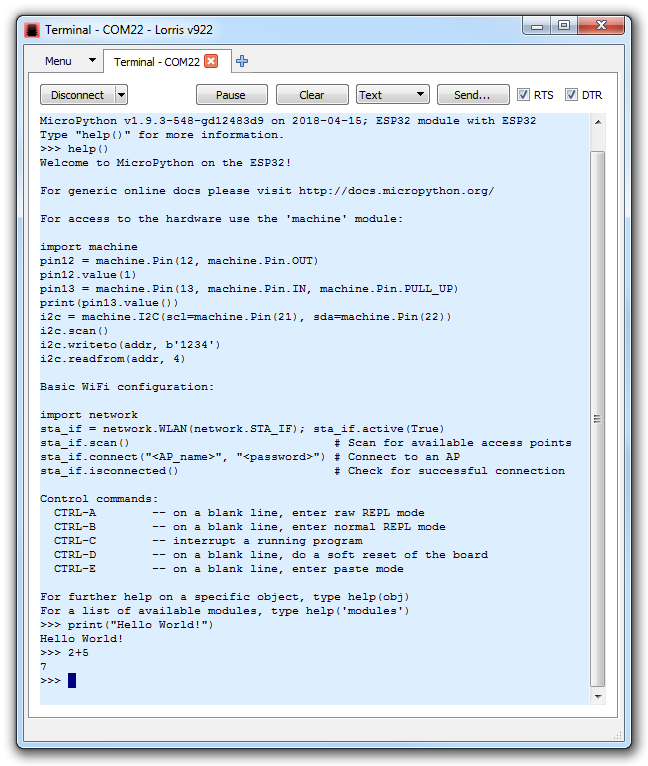
\includegraphics[width=\linewidth]{img/PythonESP.png}
\end{figure}

\subsection{Programming BMF055}
The BMF055 \cite{bosch:BMF055} is a custom programmable 9-axis motion sensor. It is a single chip triaxial accelerometer, dynamic gyroscope, magnetometer and ARM controller. The BMF055 chip is mounted on a separated board, which can be optionally mounted to the \ind{SensorBoard} or it can be used independently. The figure \ref{BMF055photo} shows the separated BMF055 board and the same board mounted to the \ind{SensorBoard}.

\begin{figure}
    \centering
    \caption{The separate BMF055 board on the left and the same board mounted to the SensorBoard on the right}
    \label{BMF055photo}
    \begin{minipage}[c]{.45\textwidth}
        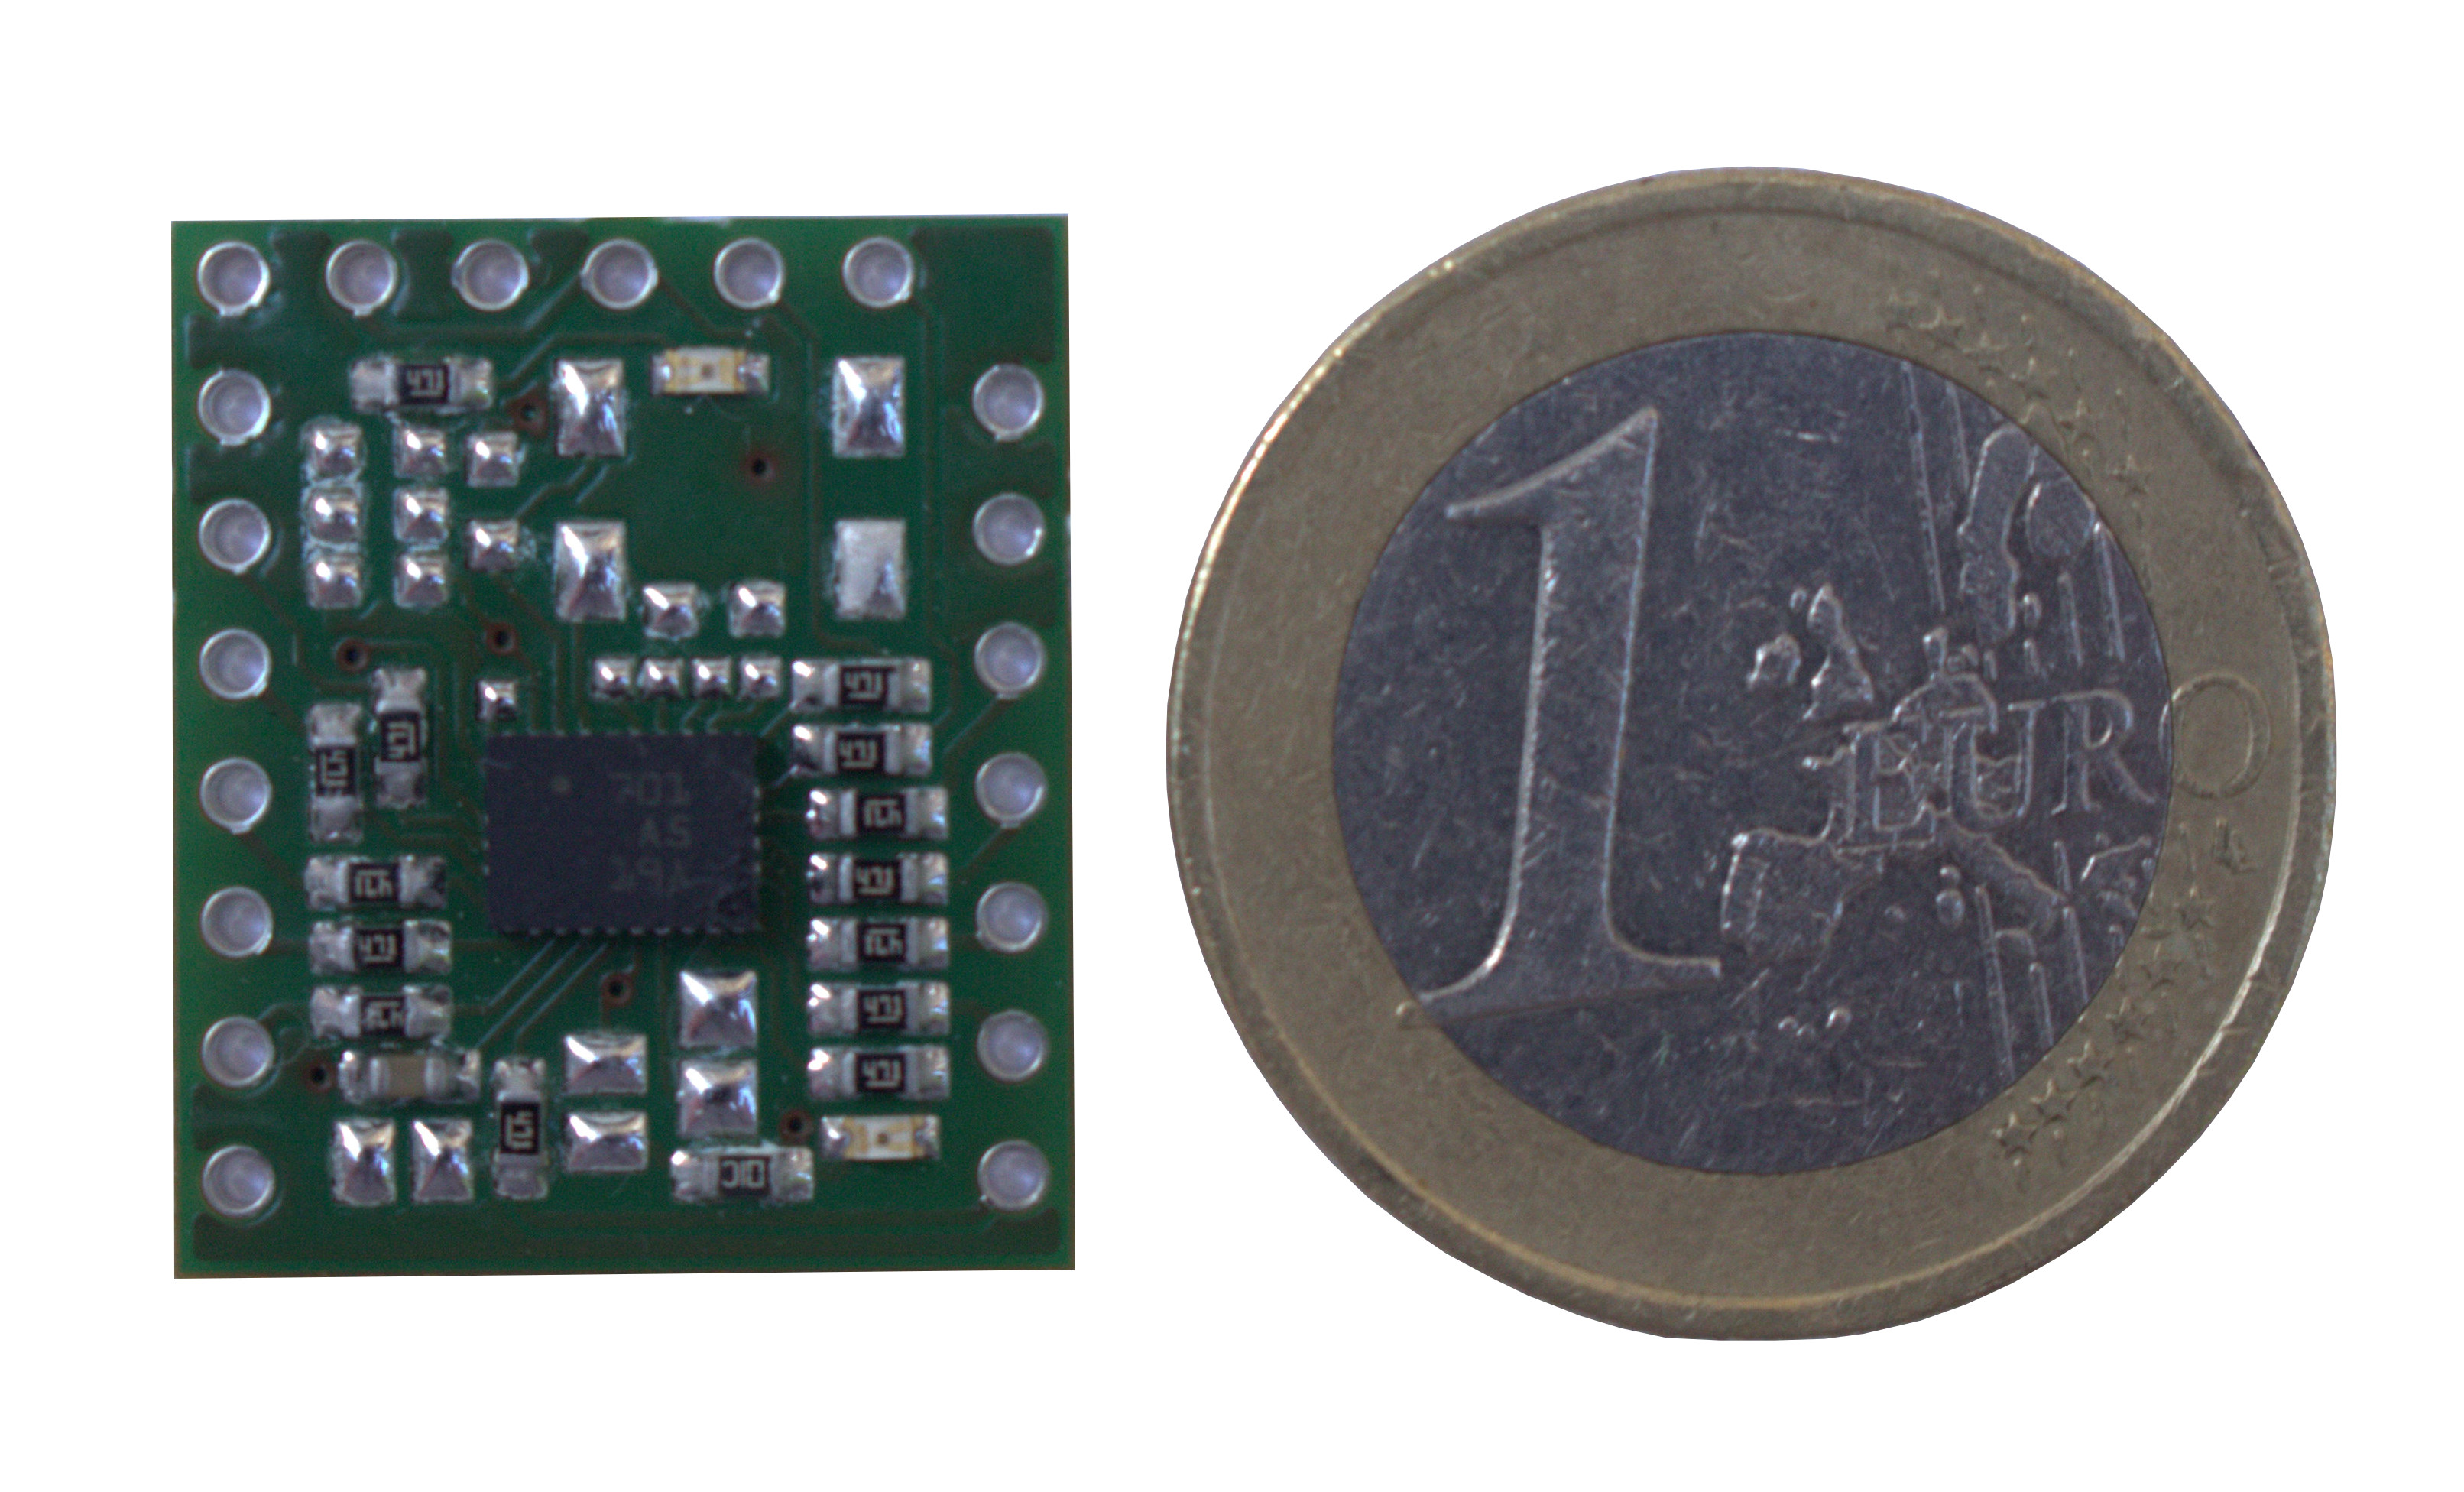
\includegraphics[width=7cm]{img/BMF055.jpg}
    \end{minipage}
    \quad\vrule{}
    \begin{minipage}[c]{.45\textwidth}
        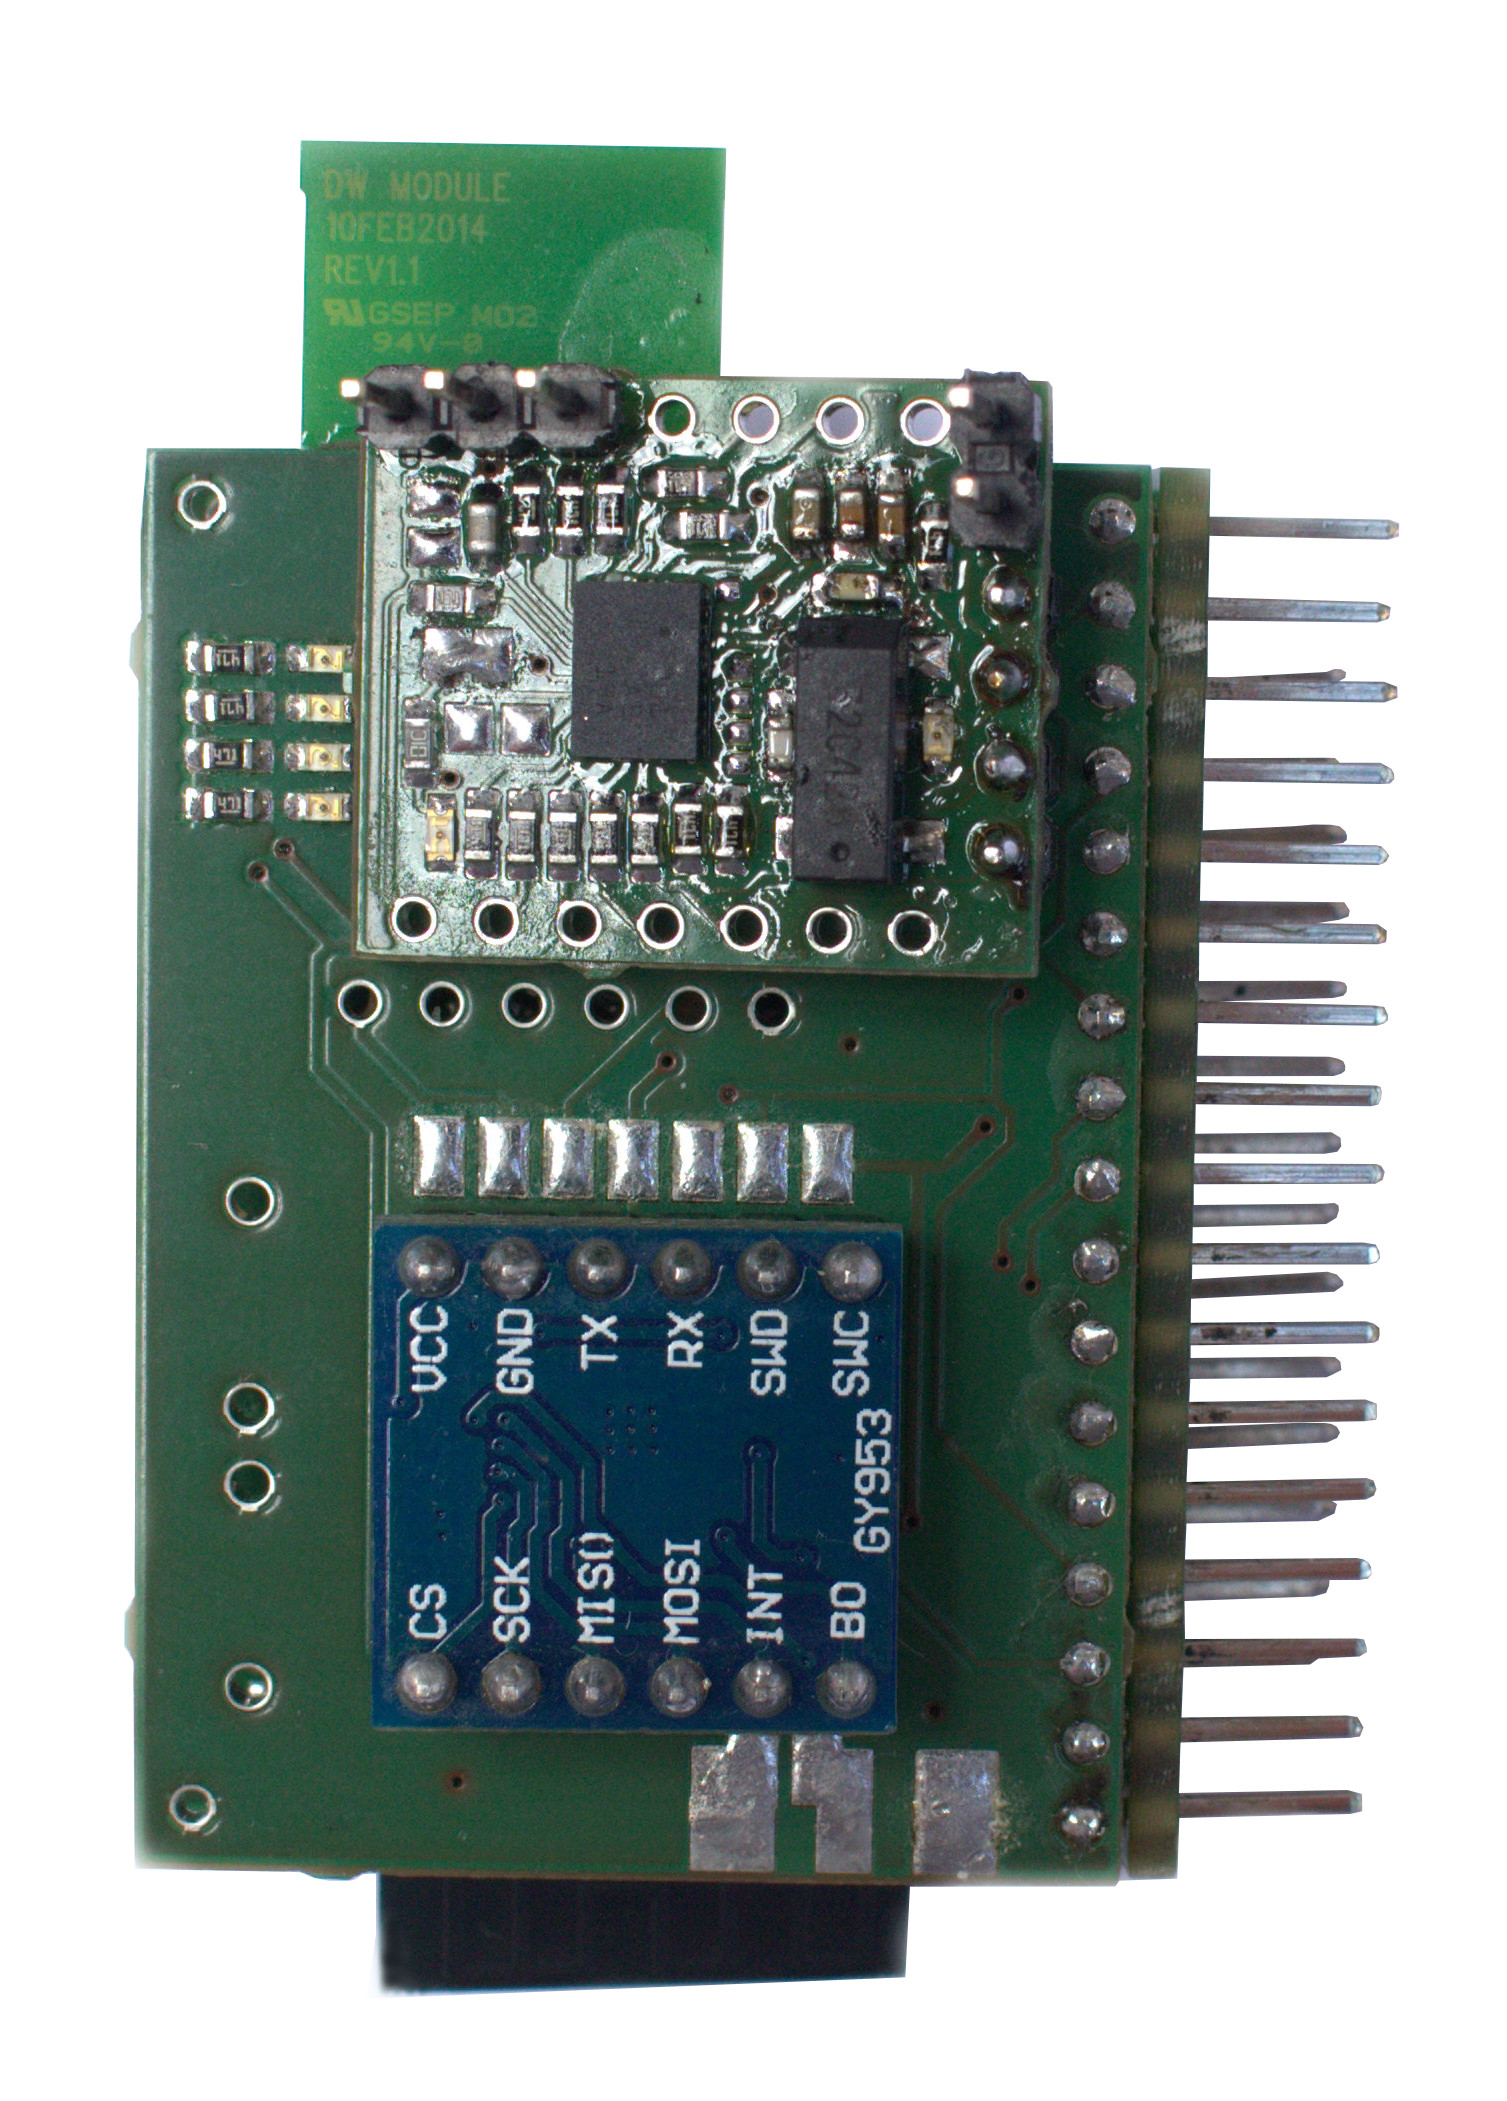
\includegraphics[width=7cm]{img/HWassembledNoCoin.jpg}
    \end{minipage}
\end{figure}

The BMF055 board has several usages because it contains a user programmable controller. It can be used for example as a simple UAV controller or autopilot. The project BMF055-flight-controller \cite{BMF055flightController} implemented an autopilot solution for multicopters on this controller.

The Atmel SAM D20 controler \cite{atmel:samd20} can be programmed in Atmel Studio \cite{AtmelStudio} and the program can be flashed to the chip via \ac{SWD} interface \cite{SWDinterface}. We have to use Atmel ICE programmer \cite{AtmelICE} or similar hardware. For details about configuration and programming of the BMF055 chip we can follow the BMF055 datasheet \cite{bosch:BMF055} or the Atmel SAM D20 datasheet \cite{atmel:samd20}. The pinout of the BMF055 board and other hardware details are described in Appendix \ref{BMF055pinNumbering}. The figure \ref{BMF055AtmelStudio} shows an opened BMF055 project in Atmel Studio 7.

\begin{figure}
    \centering
    \caption{An opened BMF055 project in Atmel Studio 7}
    \label{BMF055AtmelStudio}
    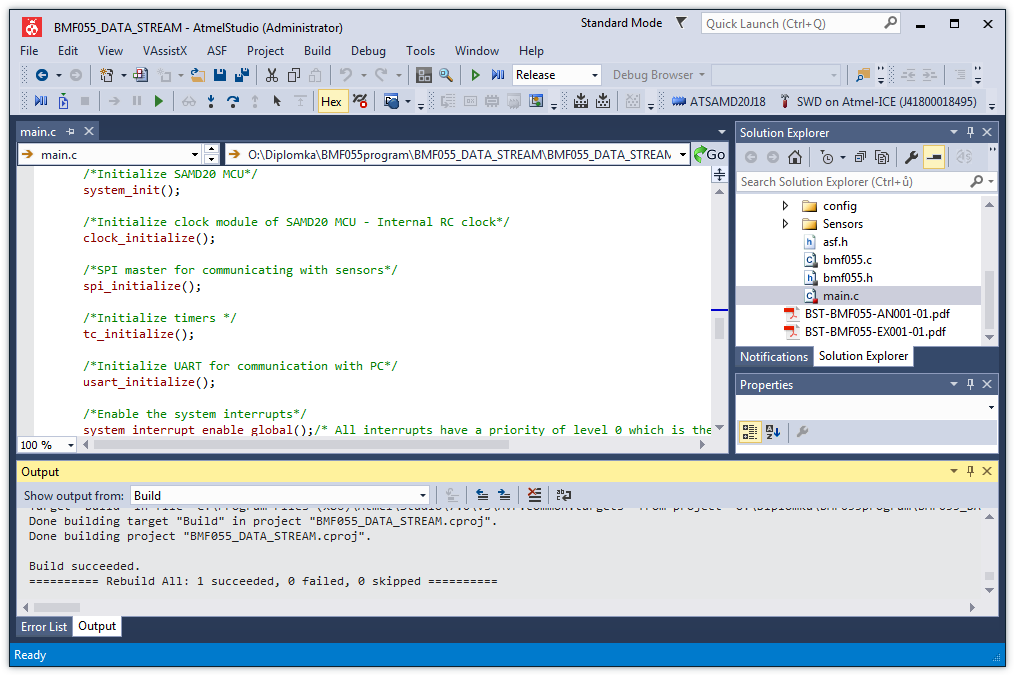
\includegraphics[width=\linewidth]{img/BMF055AtmelStudio.png}
\end{figure}

\section{Application Programming Interface (API)}
The programming interface for the \ind{SensorBoard} can be split into several categories. There is a native support from the manufacturer of the microcontrollers. This \ac{API} is written for any electronic device with the targeted microcontroller and this \ac{API} is mentioned in section \ref{GeneralAPI}.

For easier working with the sensors on the \ind{SensorBoard} I have implemented a new library. This library is described in section \ref{SensorBoardAPI}.

\subsection{SensorBoard API}
\label{SensorBoardAPI}
The \ind{ESP32} and Atmel SAM controller have defined \ac{API} by the manufacturer, but these \ac{API}s do not implement a communication with specific sensors and peripherals connected to the controllers. For easier work with all the functionality of the \ind{SensorBoard}, I have implemented specific \ac{API} for the \ind{ESP32} controller.

The \ac{API} is built on \ac{ESP-IDF} and it should be used together with the \ac{ESP-IDF} \ac{API} from the manufacturer. For example, it allows usage of a FreeRTOS, because the FreeRTOS is a part of \ac{ESP-IDF} framework \cite{espressif:ESP-WROOM-32}. The \ind{SensorBoard} \ac{API} can be used together with Arduino \ac{API} for \ind{ESP32}, too.

\paragraph{The SensorBoard \ac{API} implements}
\begin{itemize}
    \item Peripherials:
    \begin{itemize}
        \item \textbf{MPU9250} Accelerometer, dynamic gyroscope and magnetometer
        \item \textbf{BMP280} Barometer (Altitude meter)
        \item \textbf{Programmable LEDs} Two green LEDs
        \item \textbf{PWM Servo output} Controlling connected servos or regulators
        \item \textbf{File System} SD card and SPI file system
        \item \textbf{ADP5062} Battery charger and power supply configuration
        \item \textbf{Buttons} Read button state as input device
        \item \textbf{WiFi} Access Point, FTP server, remote control and communication protocol
    \end{itemize}
    \item Internal functionality:
    \begin{itemize}
        \item \textbf{Global Settings} Configuration file stored on the SD card
        \item \textbf{Stopwatch} Checking the timing of tasks
        \item \textbf{Test Sensor} Virtual sensor used for testing other functionalities
    \end{itemize}
    \item Partially implemented and actually unused
    \begin{itemize}
        \item \textbf{BMI160} Acclerometer and dynamic gyroscope
        \item \textbf{LTR-329ALS} Light sensor
        \item \textbf{SI7006} Humidity and teperature sensor
    \end{itemize}
\end{itemize}

The \ac{API} is documented in the source code and in the separate generated file.

\subsection{General \ac{API} for the controllers}
\label{GeneralAPI}
Both controllers used on the \ind{SensorBoard} have an \ac{API} defined and implemented by the manufacturer.

\newpage
\paragraph{Atmel SAM D21:} \cite{AtmelSAMd20API}
\begin{multicols}{2}
    \begin{flushleft}
        \begin{itemize}
            \setlength\itemsep{1pt}
            \item AC -- Analog Comparator (Callback \ac{API}s)
            \item ADC -- Analog-to-Digital Converter (Polled \ac{API}s)
            \item T30TSE75X Temperature Sensor
            \item AT45DBX DataFlash
            \item AVR2025 -- IEEE 802.15.4 MAC Stack v3.1.1
            \item AVR2025 -- TAL
            \item AVR2025 -- TFA
            \item AVR2025-MAC Serial Interface Module
            \item AVR2130 -- LW MESH v1.2.1
            \item BOD -- Brown Out Detector
            \item CRC-32 calculation
            \item CRC32 -- 32-bit cyclic redundancy check
            \item DAC -- Digital-to-Analog Converter (Callback \ac{API}s)
            \item Debug Print (FreeRTOS)
            \item Delay routines
            \item EEPROM Emulator Service
            \item Ethernet Physical Transceiver (ksz8851snl)
            \item EVSYS -- Event System with interupt hooks support
            \item EXTINT -- External Interrupt (Polled \ac{API}s)
            \item FatFS file system
            \item Generic board support
            \item GFX Monochrome -- Menu System
            \item GFX Monochrome -- Monochrome Graphic Library
            \item GFX Monochrome -- Spinner/Spin control widget
            \item GFX Monochrome -- System Font
            \item Interrupt management -- SAM implementation
            \item IOPORT -- General purpose I/O service
            \item Memory Control Access Interface
            \item NVM -- Non-Volatile Memory
            \item PAC -- Peripheral Access Controller
            \item Performance Analyzer Application
            \item PORT -- GPIO Pin Control
            \item QTouch Library for SAMD20/D21
            \item RTC -- Real Time Counter in Calendar Mode (Callback \ac{API}s)
            \item RTC -- Real Time Counter in Count Mode (Callback \ac{API}s)
            \item SAM D20/D21 implementation of AT25DFx SerialFlash with vectored master SPI
            \item SD/MMC stack on SPI interface
            \item SERCOM I2C -- Slave Mode I2C (Polled \ac{API}s)
            \item SERCOM SPI -- Serial Peripheral Interface (Callback \ac{API}s)
            \item SERCOM SPI -- Serial Peripheral Interface (Master Mode, Vectored I/O)
            \item SERCOM USART -- Serial Communications (Polled \ac{API}s)
            \item Serial I/O -- Host using UART
            \item Serial I/O -- NCP Using UART
            \item Sleep manager -- SAMD implementation
            \item Smart Card
            \item SSD1306 OLED controller
            \item Standard serial I/O (stdio)
            \item SYSTEM -- Clock Management for SAMD20
            \item SYSTEM -- I/O Pin Multiplexer
            \item TC -- Timer Counter (Callback \ac{API}s)
            \item Unit test framework -- SAM0 implementation
            \item USART -- Serial interface -- SAM implementation for devices with only USART
            \item WDT -- Watchdog Timer (Polled \ac{API}s)
        \end{itemize}
    \end{flushleft}
\end{multicols}

\paragraph{Espressif ESP-WROOM-32:} \cite{ESP32API}
\begin{multicols}{2}
    \begin{itemize}
        \item Wi-Fi
        \begin{itemize}
            \setlength\itemsep{1pt}
            \item Wi-Fi
            \item Smart Config
            \item ESPNOW
        \end{itemize}
        \item Mesh
        \begin{itemize}
            \setlength\itemsep{1pt}
            \item ESP Mesh
        \end{itemize}
        \item Bluetooth
        \begin{itemize}
            \setlength\itemsep{1pt}
            \item Bluetooth Controller \&\& VHCI
            \item Bluetooth Common
            \item Bluetooth LE
            \item Bluetooth Classic
        \end{itemize}
        \item Ethernet
        \begin{itemize}
            \setlength\itemsep{1pt}
            \item Ethernet
        \end{itemize}
        \item Peripherals
        \begin{itemize}
            \setlength\itemsep{1pt}
            \item ADC
            \item DAC
            \item GPIO (including RTC low power I/O)
            \item I2C
            \item I2S
            \item LED Control
            \item MCPWM
            \item Pulse Counter
            \item Remote Control
            \item SDMMC Host
            \item SD SPI Host
            \item Sigma-delta Modulation
            \item SPI Master
            \item SPI Slave
            \item Timer
            \item Touch Sensor
            \item UART
        \end{itemize}
        \item Protocols
        \begin{itemize}
            \setlength\itemsep{1pt}
            \item mDNS
            \item ESP-TLS
        \end{itemize}
        \item Storage
        \begin{itemize}
            \setlength\itemsep{1pt}
            \item SPI Flash and Partition \ac{API}s
            \item SD/SDIO/MMC Driver
            \item Non-Volatile Storage
            \item Virtual Filesystem
            \item FAT Filesystem
            \item Wear Levelling
            \item SPIFFS Filesystem
        \end{itemize}
        \item System
        \begin{itemize}
            \setlength\itemsep{1pt}
            \item FreeRTOS
            \item FreeRTOS Hooks
            \item Heap Memory Allocation
            \item Heap Memory Debugging
            \item Interrupt Allocation
            \item Watchdogs
            \item Inter-Processor Call
            \item High Resolution Timer
            \item Logging
            \item Application Level Tracing
            \item Power Management
            \item Sleep Modes
            \item Base MAC address
            \item Over The Air Updates (OTA)
            \item ESP pthread
        \end{itemize}
        \item Configuration Options
        \begin{itemize}
            \setlength\itemsep{1pt}
            \item Kconfig
        \end{itemize}
    \end{itemize}
\end{multicols}

\section{Usage Examples}
The \ind{SensorBoard} is a multifunctional user programmable hardware that can be used in several ways. There are some examples presented in this section.

\subsection{Sensors data logger}
\label{ExampleLogger}
Sensor logger can be understood as very simple logging device or as a very advanced application with an integrated web server and with the ability to connect more boards into one synchronized grid with centralized control. The simple version is shown in figure \ref{UELogging1}.

\begin{figure}
    \centering
    \caption{Simple logging application with SensorBoard}
    \label{UELogging1}
    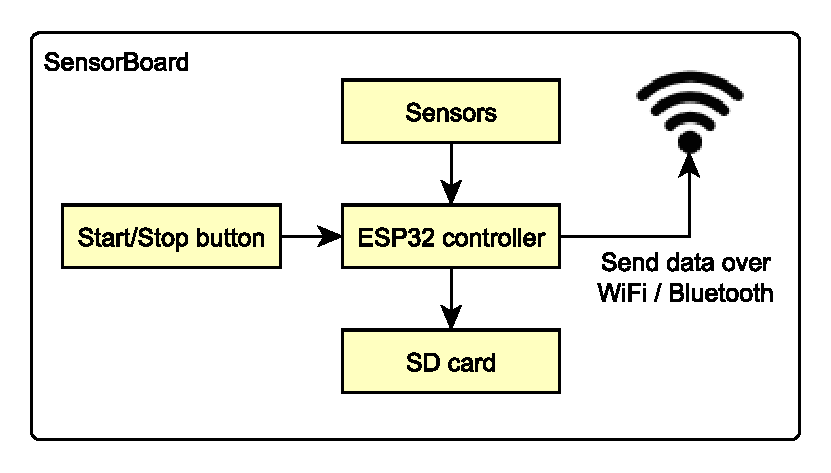
\includegraphics[scale=1]{img/UsageExamplesLogger1.pdf}
\end{figure}

When we need to measure some inertial data, we sometimes need more sensors placed in different places of the analyzed object. Tt is a big advantage when we can start and stop all the sensors synchronously and control all of them by one button. This solution is shown in figure \ref{UELogging2}.

\begin{figure}
    \centering
    \caption{Advanced logging application with SensorBoard}
    \label{UELogging2}
    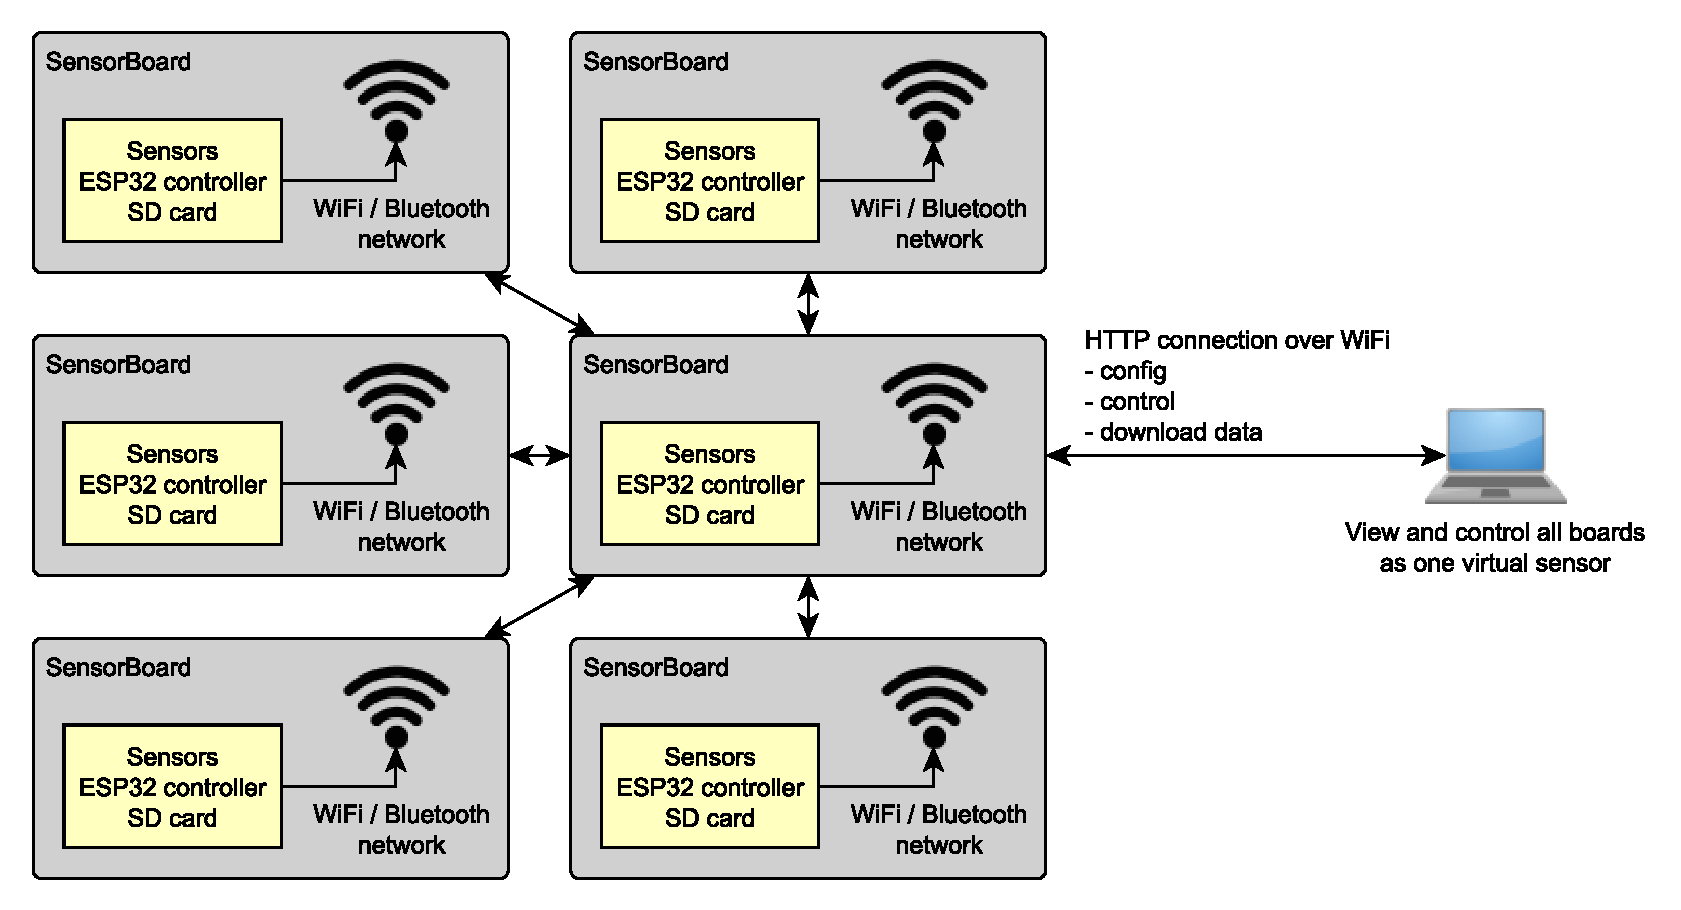
\includegraphics[width=\linewidth]{img/UsageExamplesLogger2.pdf}
\end{figure}

I am using this advanced configuration during the analysis of a movement of a horse. This solution is explained in detail in section \ref{HorseFirmware}. The goal of this task is how to recognize the type of the movement of a horse (stand, walk, trot, canter or gallop). We can get some results from only one sensor, but we get more accurate results when we can measure each leg and the other places on the horse's body separately. How the \ind{SensorBoard}s are used in this task is shown in figure \ref{UELoggingHorse}.

\begin{figure}
    \centering
    \caption{Configuration of the SensorBoard on a horse}
    \label{UELoggingHorse}
    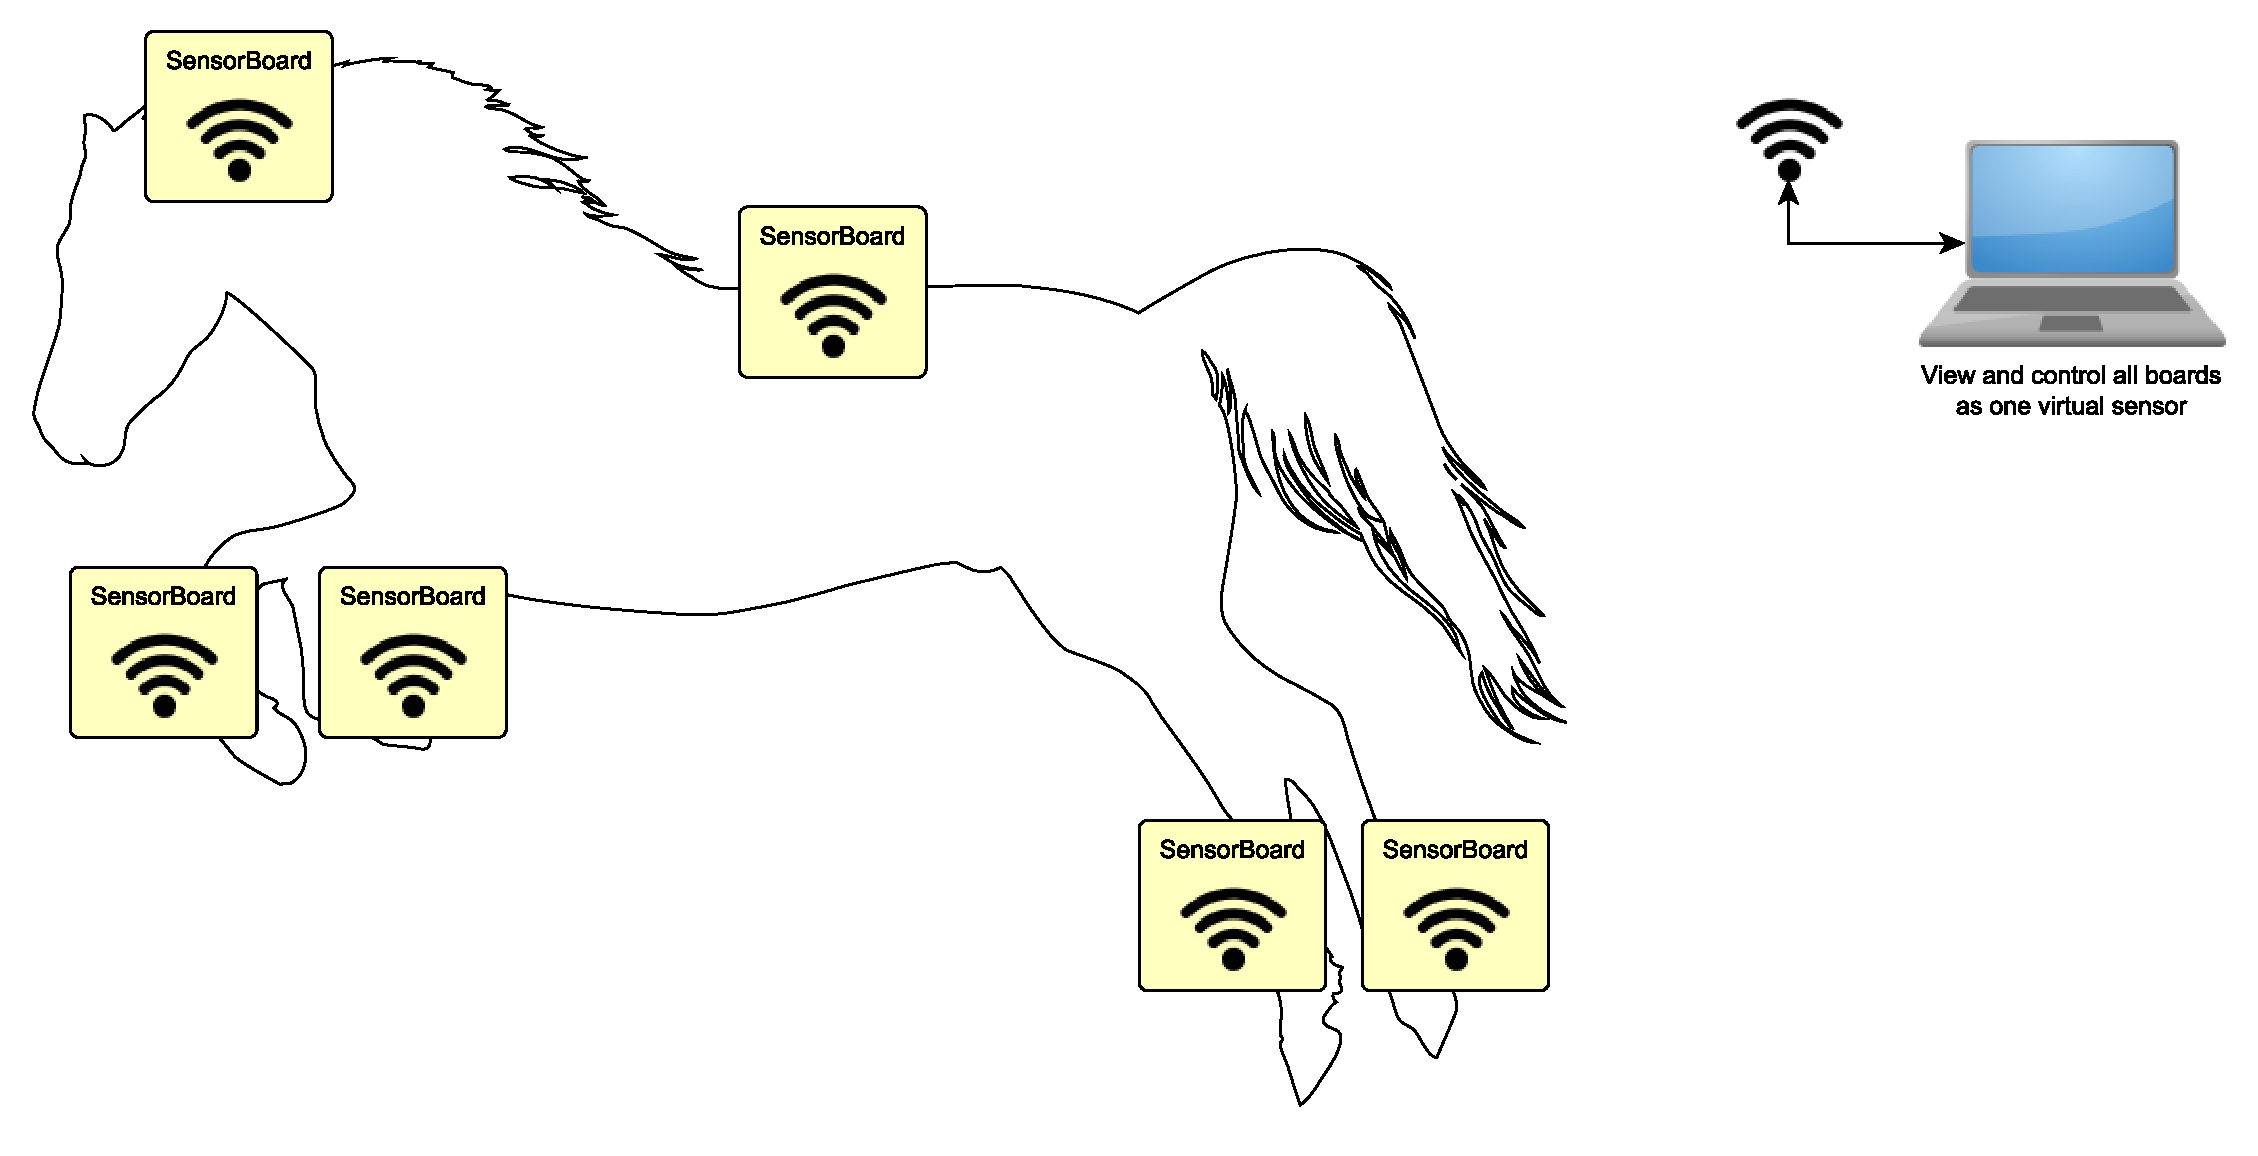
\includegraphics[width=\linewidth]{img/UsageExamplesLoggerHorse.pdf}
\end{figure}

\subsection{Sensor fusion and \ac{AHRS}}
\label{ExampleAHRS}
Sensor fusion \index{sensor fusion} is a method that combines data from more sensors and calculates a~new information. The new information is read from the \ind{sensor fusion} algorithm like from a~virtual sensor. \cite{SensorFusion}

This example shows how to use a \ind{sensor fusion} algorithm for computing \ac{AHRS} data on the \ind{SensorBoard}. \ac{AHRS} is Attitude and Heading Reference System and computes pitch, roll and yaw values from the triaxial accelerometer, dynamic gyroscope and magnetometer data. We can use for example Madgwick's algorithm \cite{MadgwickAHRS} in the way shown in figure \ref{UEAHRS}. This application is the base step for example \ref{ExampleBMF055FlightController}.

\begin{figure}
    \centering
    \caption{Sensor fusion example on custom \ac{AHRS}}
    \label{UEAHRS}
    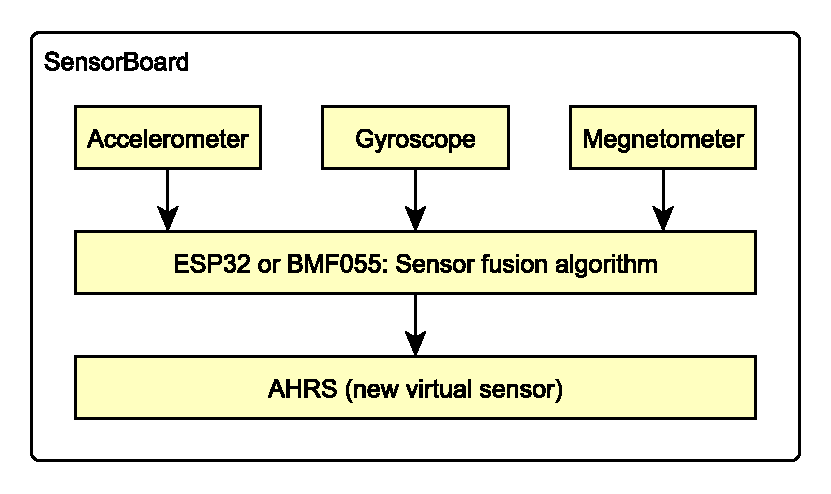
\includegraphics[scale=1]{img/UsageExamplesAHRS.pdf}
\end{figure}

We can use an advantage of two controllers at one board and run the \ind{sensor fusion} algorithm on the BMF055 chip and the \ind{ESP32} is still free for some user program like is shown in figure \ref{UEAHRSBMF}. When an error occurs in the user program, the \ind{sensor fusion} at BMF055 chip continues to run without any problem. This feature is a big advantage for Flight Controllers where we want to allow the user to run for example his navigation code.

\begin{figure}
    \centering
    \caption{Sensor fusion \ac{AHRS} example with two controllers}
    \label{UEAHRSBMF}
    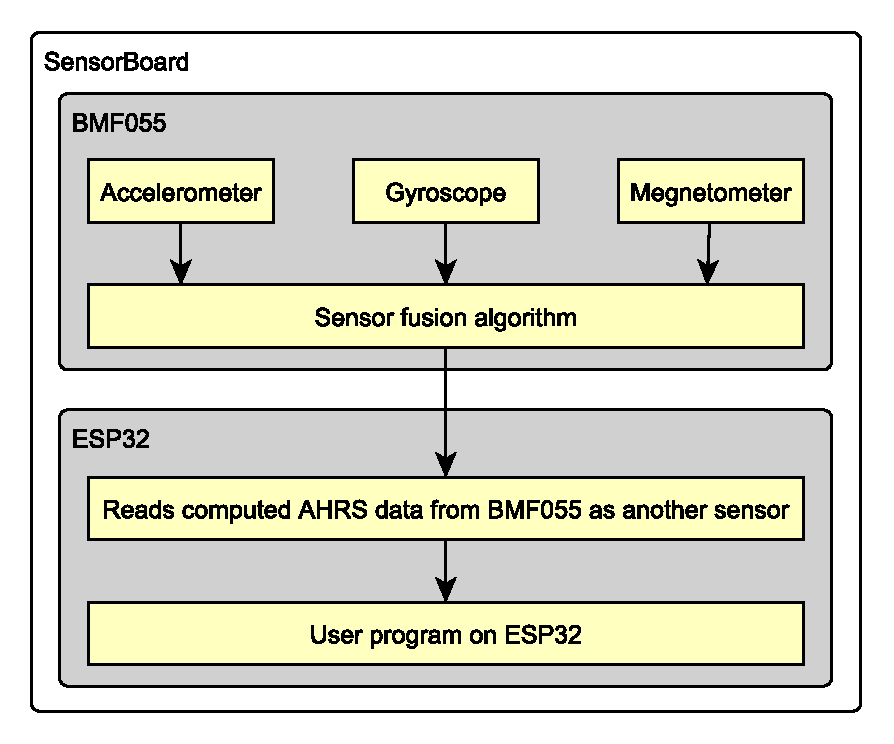
\includegraphics[scale=1]{img/UsageExamplesAHRSBMF.pdf}
\end{figure}

\subsection{UAV Flight controller with non-critical user programmable processor}
\label{ExampleBMF055FlightController}
The \index{flight controller}s must be very reliable devices. They usually consist of two parts. The first part controls the pitch, roll, yaw, velocity, the angle of attack etc. The second part is a navigator that processes user commands and makes high-level flight planning. The pilot's input can be processed on both parts. We usually want to create only the basic control algorithm, which is safety critical, and develop all the remaining parts as a non-critical code.

Here we can use dual controller advantage on the \ind{SensorBoard} and run the basic critical code at the first controller and the remaining non-critical code on the second controller. The non-critical program on the second controller is usually a navigator or user program. The figure \ref{UEFlightController} shows the possible configuration of the flight controller on the \ind{SensorBoard}. This configuration uses BMF055 Flight Controller \cite{BMF055flightController} by Lukas Blocher. His code can be compiled directly for the \ind{SensorBoard} without any modification.

\begin{figure}
    \centering
    \caption{SensorBoard used as a quadcopter flight controller}
    \label{UEFlightController}
    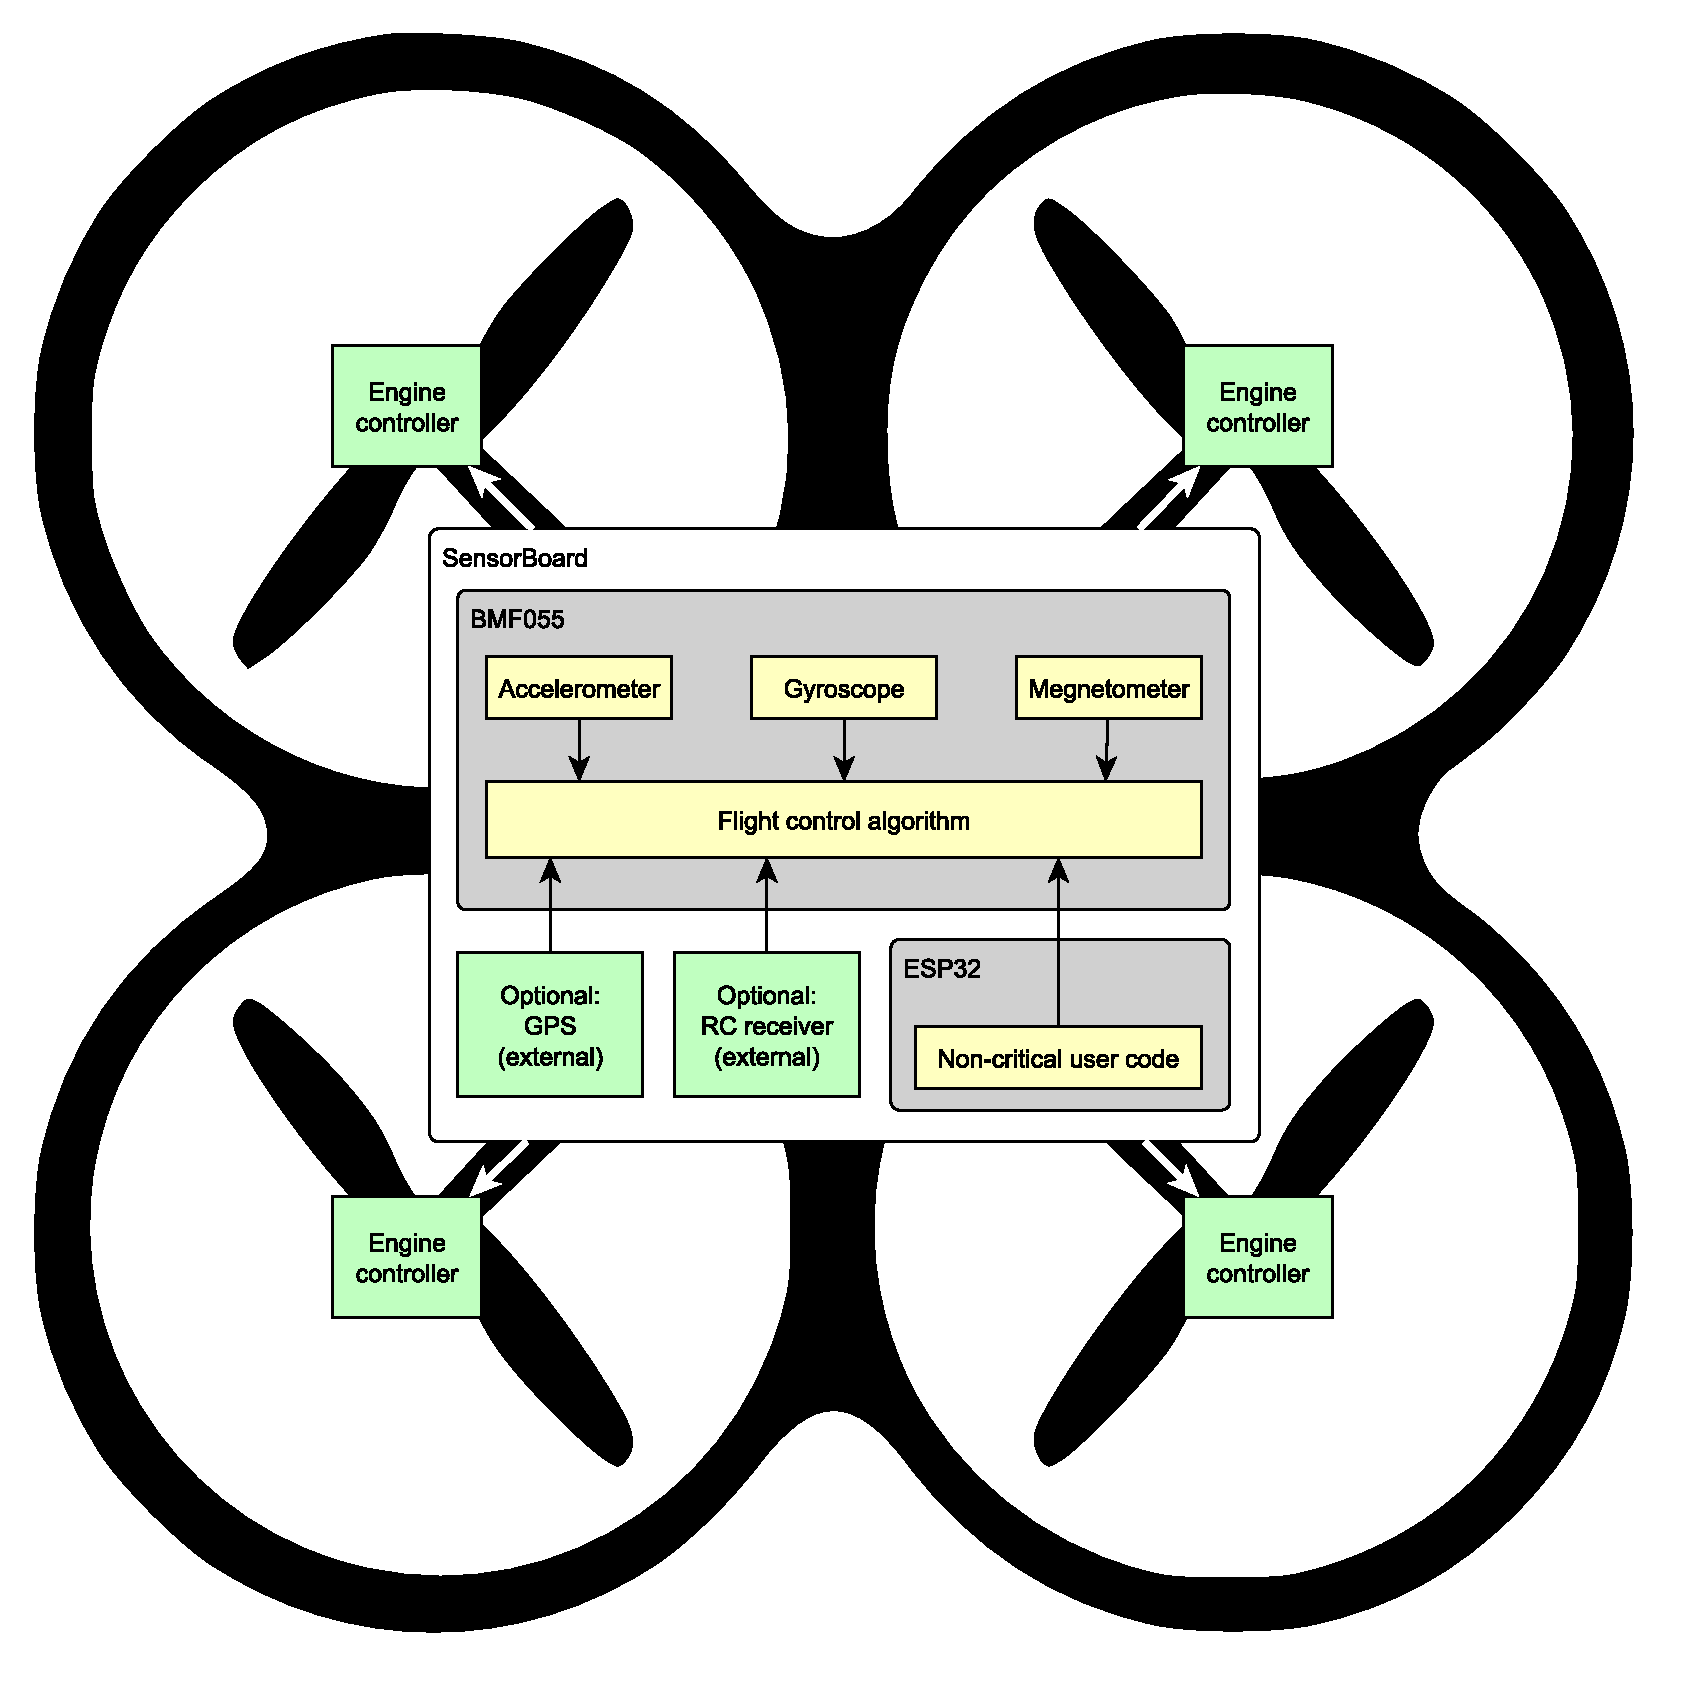
\includegraphics[width=\linewidth]{img/UsageExamplesFlightController.pdf}
\end{figure}

\subsection{Indoor navigation using \ac{TDOA}}
Indoor navigation requires high accuracy positioning. We usually need a higher accuracy than given by GPS. I know many projects approaching the indoor positioning. For example, there was an \ind{Indoor Positioning} and \ind{Indoor Navigation} conference in September 2017 in Japan.

This example uses Time Difference of Arrival (\ac{TDOA}) method to compute its position in space with the precision of \SI{10}{cm}. The device measures time differences in received messages from other devices. When the device knows the time differences and the speed of light, it can compute its relative position to the other boards. There is a DWM1000 chip that is able to measure and compute these data. \cite{decawave:DWM1000}. The figure \ref{UETDOA} shows how the relative positioning works on the \ind{SensorBoard}.

\begin{figure}
    \centering
    \caption{\ac{TDOA} relative location service on the SensorBoard}
    \label{UETDOA}
    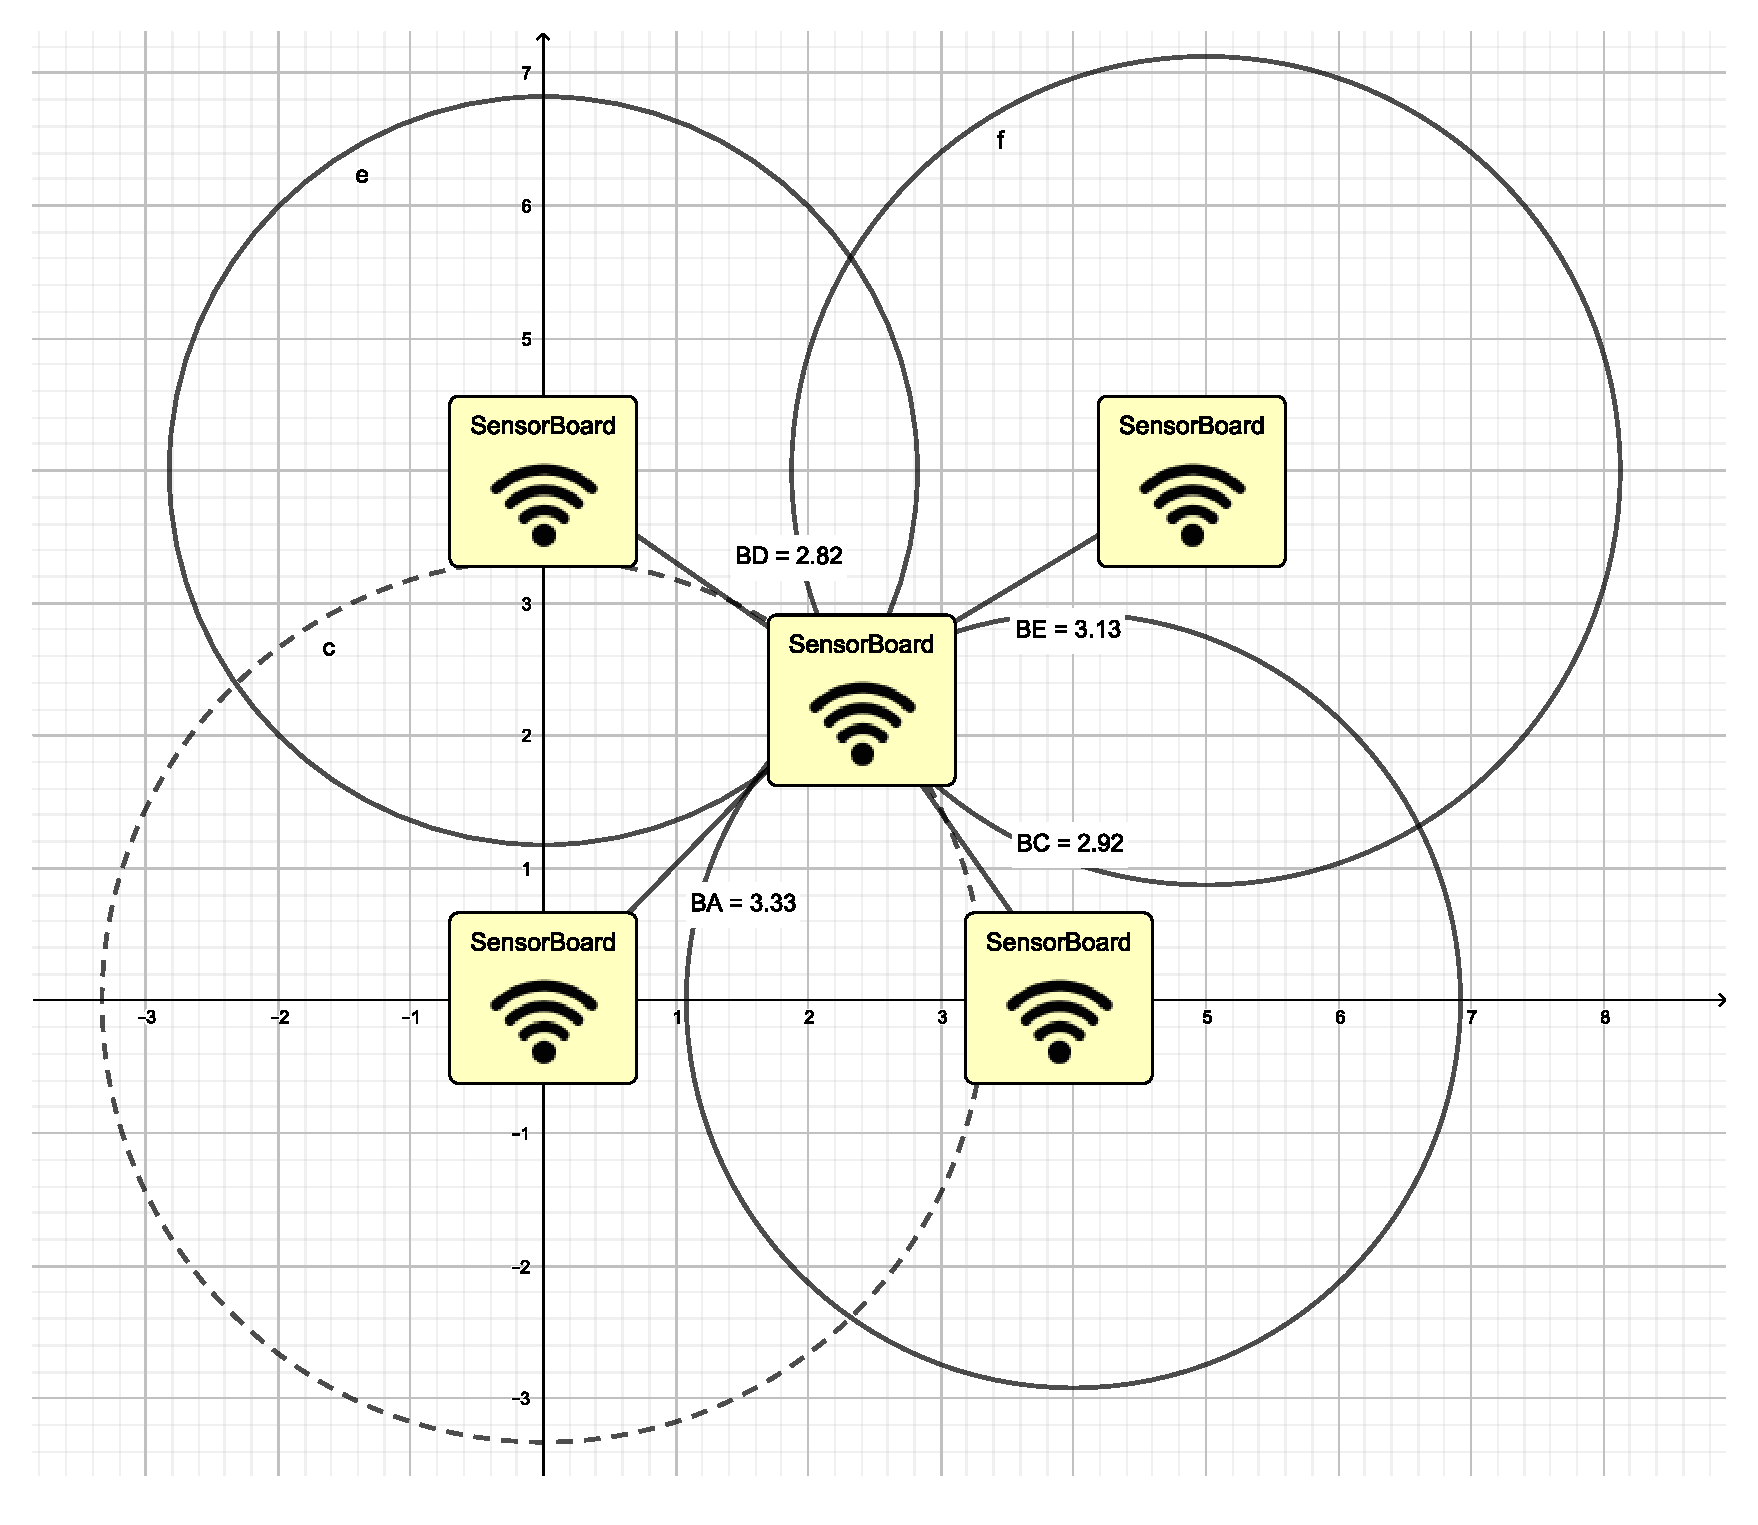
\includegraphics[trim=5cm 6cm 5cm 5cm, clip, width=15cm]{img/UsageExamplesTDOA.pdf}
\end{figure}

The DWM1000 \cite{decawave:DWM1000} module is present on the \ind{SensorBoard} and when it connects to at least three other boards, it computes its relative position with the mentioned precision. When the board knows an absolute position of the other boards, it can compute its absolute position, too. The absolute location can be obtained for example from GPS receiver or from static transmitters.

When we use the \ac{AHRS} mentioned in section \ref{ExampleAHRS}, we have all data about current position and attitude of the \ind{SensorBoard}. We can use some other sensors on the \ind{SensorBoard} like BMP280 barometer \cite{bosch:BMP280} to improve the current position and attitude data.

\subsection{RTOS education board}
Real-time systems are different from common operating systems in personal computers and they cannot be emulated as a standard application for a computer with the common operating system. The common operating system does not give a guarantee that a job completes on time, so any application running on this operating system cannot give this guarantee, too.

The \ind{ESP32} controller on the \ind{SensorBoard} uses FreeRTOS and supports all its functionality. \cite{ESP32FreeRTOS} We can run a hard real-time system on the \ind{SensorBoard} or on the other hand, we can use the \ind{SensorBoard} for education about real-time systems. Simple FreeRTOS application uses only the \ind{ESP32} controller like is shown in figure \ref{UEFreeRTOS} and optionally we can use the sensors as data sources and as resources.

\begin{figure}
    \centering
    \caption{FreeRTOS application diagram on ESP32 on the SensorBoard}
    \label{UEFreeRTOS}
    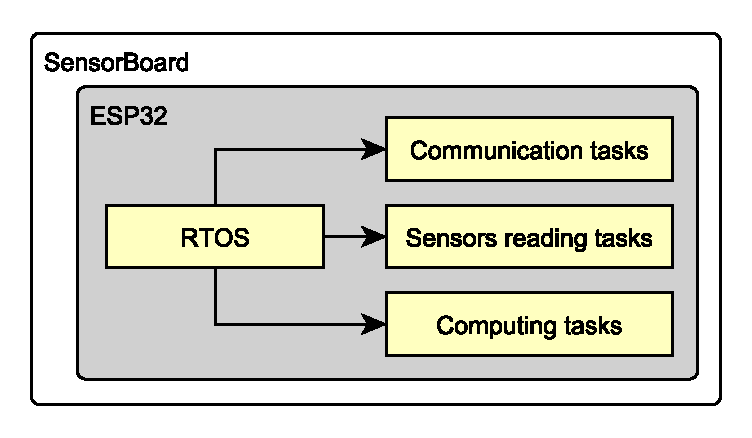
\includegraphics[scale=1]{img/UsageExamplesRTOS.pdf}
\end{figure}

\subsection{MicroPython Robot Controller}
The \ind{SensorBoard} supports MicroPython firmware \cite{MicroPython} on the \ind{ESP32} controller. When we create a Python library that implements simple \ac{API} for controlling some electromechanical device. We can use the \ind{SensorBoard} as a controller of this electromechanical hardware. Then we simply send Python commands via UART or WiFi to the target device.

In my opinion, this setup is an easy way how to teach students the basics of programming (in Python) with some dynamic hardware. This way of teaching is probably easier for the students and it probably creates more interactivity between students and the device. The figure \ref{UEMicroPython} shows an example of using MicroPython inside the \ind{SensorBoard}.

\begin{figure}
    \centering
    \caption{MicroPython robot controller example on the SensorBoard}
    \label{UEMicroPython}
    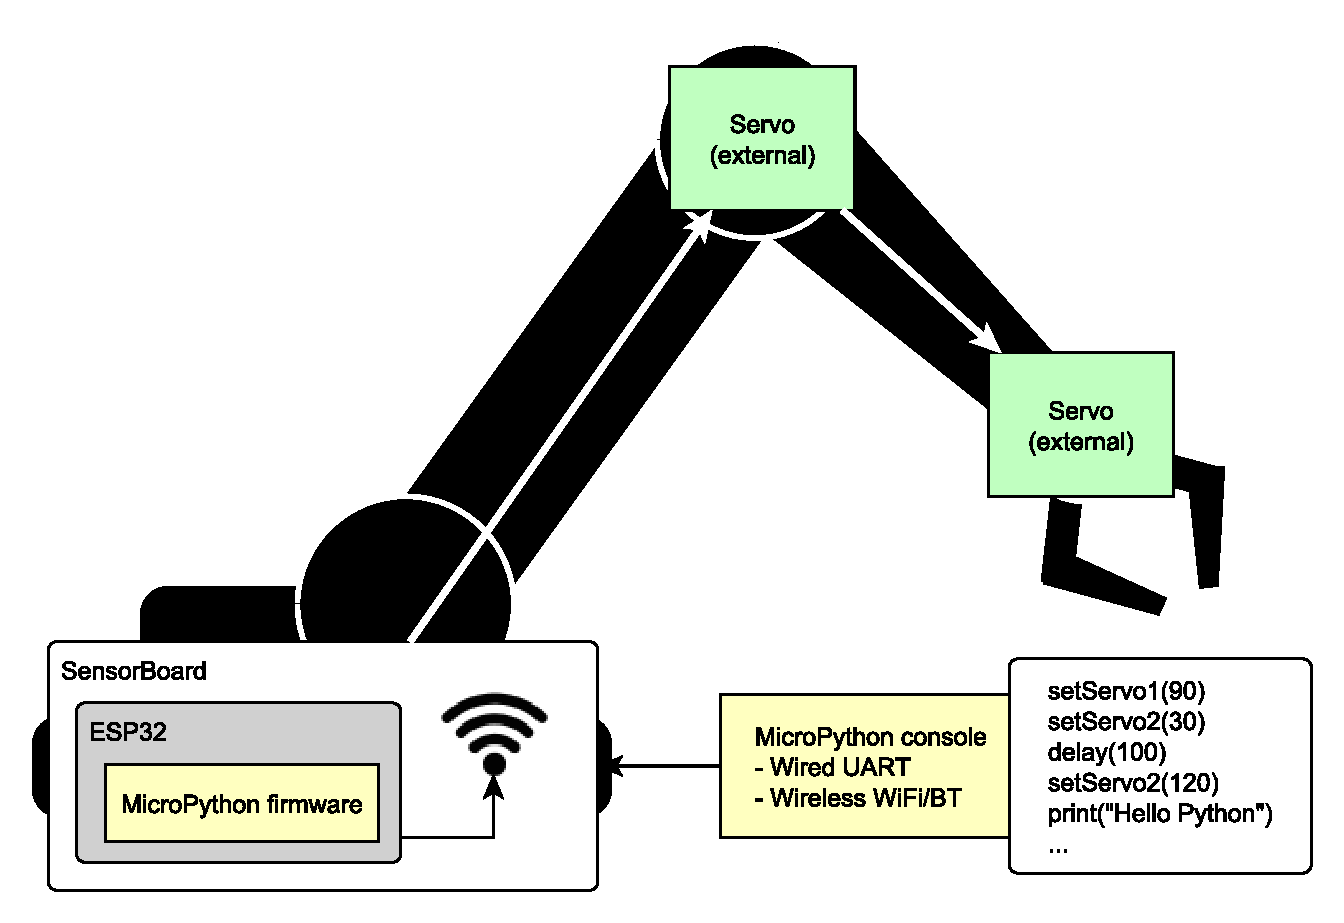
\includegraphics[width=\linewidth]{img/UsageExamplesPythonRobot.pdf}
\end{figure}

\subsection{WiFi AccessPoint with server services}
The \ind{ESP32} controller has a built-in Bluetooth and WiFi module. So, we can create any WiFi based application on the \ind{SensorBoard}. The only limitation is memory (SD card up to \SI{32}{GB}) and CPU power (dual-core \SI{240}{MHz}). We can use the \ind{SensorBoard} for example as a simple HTTP server \cite{ESP32:HTTPserver} or FTP server \cite{ESP32:FTPserver} or implement any other WiFi-based service like is shown in figure \ref{UEWiFi}.

\begin{figure}
    \centering
    \caption{WiFi based services example on the SensorBoard}
    \label{UEWiFi}
    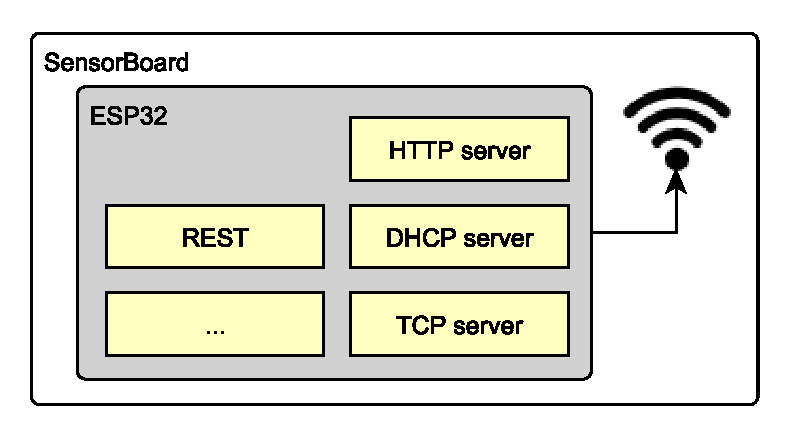
\includegraphics[scale=1]{img/UsageExamplesServer.pdf}
\end{figure}

\subsection{Grid computing education board}
\label{ExampleGrid}
The biggest advantages of the \ind{SensorBoard} are hidden in its real-time system, wireless technology and independence. These advantages can create a grid of multiple items. We can use the whole grid as one virtual unit. When we solve the problems with failures and accessibility, we have a grid with swappable items. An example of a grid with two failures is shown in figure \ref{UEgrid}.

\begin{figure}
    \centering
    \caption{Example of a grid with two failures created from multiple SensorBoards}
    \label{UEgrid}
    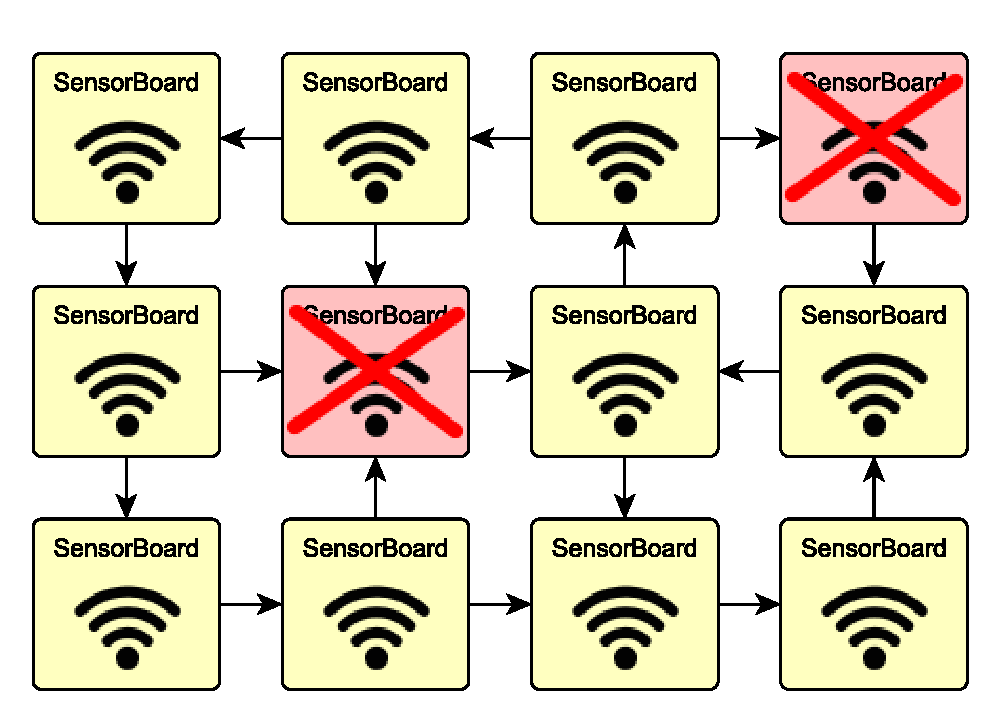
\includegraphics[width=\linewidth]{img/UsageExamplesGrid.pdf}
\end{figure}

\subsection{\ac{IoT} wireless sensors}
The Internet of Things (\ac{IoT}) is a commercially used word for all devices connected to the Internet with some sensors onboard. The \ind{SensorBoard} fulfills both conditions and it can be used directly this way. The figure \ref{UEIoT} shows an example of using the \ind{SensorBoard} as a device reading sensors data and streaming them via GSM network or via WiFi connection.

\begin{figure}
    \centering
    \caption{Example of using SensorBoard as an \ac{IoT} device streaming data from sensors via WiFi or GSM network}
    \label{UEIoT}
    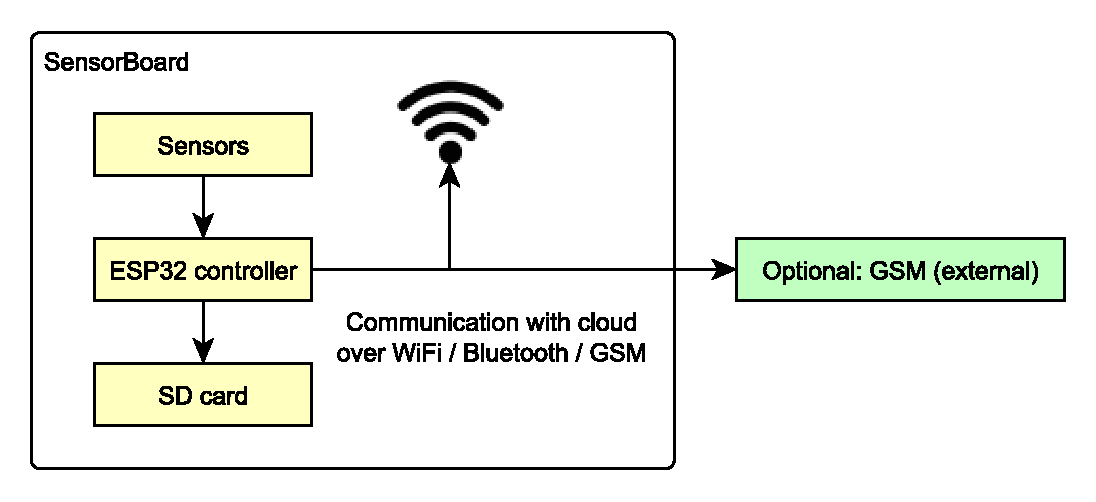
\includegraphics[width=\linewidth]{img/UsageExamplesIoT.pdf}
\end{figure}

\section{Movement Analysis Firmware}
\label{HorseFirmware}
The firmware is a sensor data logging application similar to the example in section \ref{ExampleLogger}. The program is able to read values from sensors in a defined frequency and store the captured data to SD card and/or send them directly via WiFi. The application is controlled by start/stop button or via \ac{TCP} connection.

When the \ind{SensorBoard} is switched on, it initializes WiFi access point and waits 5~seconds before the reading and logging procedure starts. After these 5 seconds, the board enters a loop and starts logging data to SD card. The logging loop can be stopped via \ac{TCP} connection, by pressing the start/stop button or by switching the board off.

When we want to control the \ind{SensorBoard} via \ac{TCP} client, we have to connect our device to \ind{SensorBoard}'s WiFi access point. Then we can connect to the \ac{TCP} server and send the control commands.

\subsection{Before first use}
\label{beforeFirstUse}
All the configuration is saved in \texttt{config.ini} file on the SD card (root directory). The configuration is read whenever the \ind{SensorBoard} is powered on. The configuration file is never modified by the \ind{SensorBoard}. An example of the configuration file is in figure \ref{SBconfigFile}. If no configuration file is present on the SD card, default values are used.

\begin{figure}
    \centering
    \caption{Example of the configuration file on SD card}
    \label{SBconfigFile}
    \begin{verbatim}
    % Enable or disable WiFi adapter
    isWiFienabled = true
    
    % Initializes WiFi as an access point when true,
    % otherwise as a station
    isWiFiAccessPoint = true
    
    % Network SSID
    % When initialized as AP: creates the new network
    WiFiSSID = SensorBoard
    
    % WiFi network password
    WiFiPassword = 1234567890
    
    % IP address of the device,
    myIP = 192.168.1.1
    
    % TCP server port
    TCPseverPort = 3000
    
    % If enabled, starts logging automatically 'startUpWaitTime' seconds
    % after powered on
    startLoggingImmediately = true
    
    % Waits N milliseconds before entering the logging loop
    startUpWaitTime = 5000
    
    % If enabled, the horse movement analysis starts automatically
    isHorseAnalysis = false
    
    % If enabled, the data streaming starts automatically
    isStreaming = false
    
    % If enabled, the logging can be controlled by the start/stop button
    isStartButtonUsed = false
    
    % Log file name for sensor data,
    % a number prefix is automatically added
    logFileName = log.csv
    
    % Log file name for movement analysis,
    % a number prefix is automatically added
    horseAnalysisFileName = horse.txt
    \end{verbatim}
\end{figure}

\subsection{Files on the SD card}
All the files are stored and read from the root directory of the SD card. The files are:

\begin{itemize}
    \item \textbf{config.ini}: (read-only) Configuration file explained in section \ref{beforeFirstUse}.
    \item \textbf{counter.txt}: (read/write) This text file contains only one integer on the first line, other data are ignored. The \ind{SensorBoard} has no real-time clock reference, so it cannot add a timestamp to each log file. The board increments this number after each startup. This number is used as session number of each log file.
    \item \textbf{X\_Y\_log.csv}: (write only) The main log file in CSV format. The name consists of the session number \texttt{X}, log number \texttt{Y} and the configured filename. The format is \texttt{X\_Y\_NAME}, for example \texttt{12\_34\_log.csv}. It means that the file was created after 12th switching on, it is 34th log during the session and the configured file name is \texttt{log.csv}.
    \item \textbf{format.txt} (write only) Format of the CSV main log file. This file contains names of all columns in order in the main log file. Example of this file is shown in figure \ref{formatFile}.
    \item \textbf{X\_Y\_horse.txt}: (write only) The movement analysis log file in plain text or CSV format. The \texttt{X}, \texttt{Y} numbers correspond to the main log file numbers. The files with the same numbers were captured simultaneously during the same measurement.
\end{itemize}

\begin{figure}
    \centering
    \caption{Example of the 'format.txt' file on SD card.}
    \label{formatFile}
    \begin{verbatim}
    'S'; #; milliseconds; baroAltitude QFE [m]; baroTemp [degree C];  \
    ACC_X [g]; ACC_Y [g]; ACC_Z [g];                                  \
    GYR_X [rad/s]; GYR_Y [rad/s]; GYR_Z [rad/s];                      \
    MAG_X [degree];  MAG_Y [degree];  MAG_Z [degree];                 \
    ...
    \end{verbatim}
\end{figure}

\subsection{Using the firmware}
The application is usually used only during the measurement process. The behavior of the program can be described using the state machine presented in figure \ref{firmwareStateMachine}.

\begin{figure}
    \centering
    \caption{State machine of the firmware}
    \label{firmwareStateMachine}
    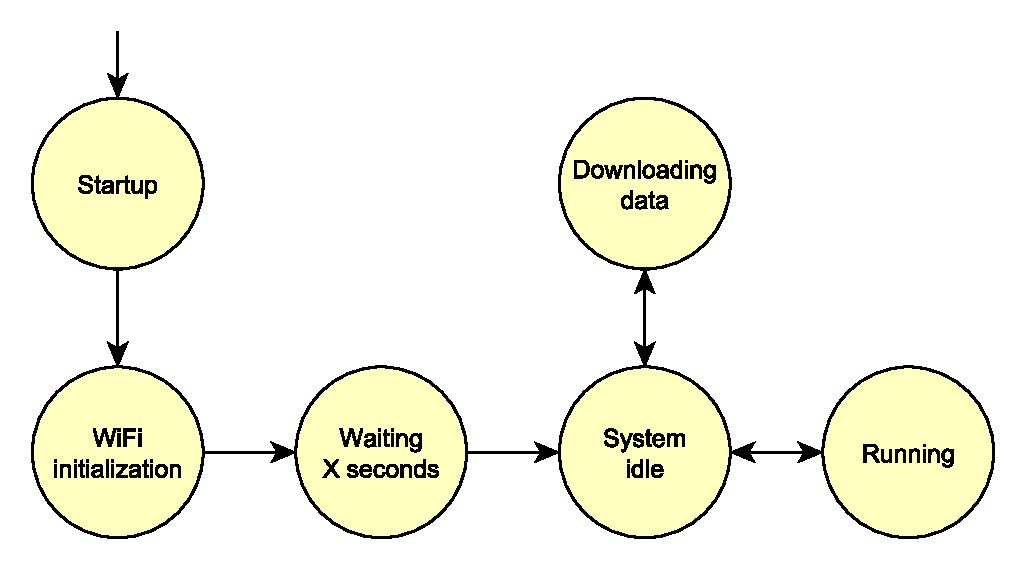
\includegraphics[width=\linewidth]{img/firmwareStateMachine.pdf}
\end{figure}

The meaning of each state of the machine:
\begin{itemize}
    \item \textbf{Startup} Powering on the board
    \item \textbf{WiFi initialization} Initialization of the WiFi adapter according to the configuration file
    \item \textbf{Waiting N seconds} Waiting a few (milli)seconds according to the configuration file. We usually configure this waiting when we want to prevent the creation of very short logs.
    \item \textbf{System idle} The system is waiting for control commands. If the board is configured to start logging immediately, the system automatically switches to running state.
    \item \textbf{Downloading data} The data can be downloaded directly from the SD card or to a connected device.
    \item \textbf{Running} The Running state starts the measuring loop and allows to log, stream or analyze the measured data. It is not possible to download data from SD card in this state. This state is activated when the user starts logging, streaming or movement analysis process from the Idle state. The Running state can be activated automatically according to the configuration file.
\end{itemize}

\subsection{Horse movement analysis feature}
The application has built-in movement analysis tool. When the \ind{SensorBoard} is placed on a horse's body, the tool can determine when the horse is moving and what kind of movement it does. The figure \ref{fig:HorseAnalysisTablet} shows a screenshot from the tablet used for controlling the \ind{SensorBoard} during measurement process on a horse's body.

\begin{figure}
    \centering
    \caption{Screenshot from the tablet used for controlling the SensorBoard during measurement process}
    \label{fig:HorseAnalysisTablet}
    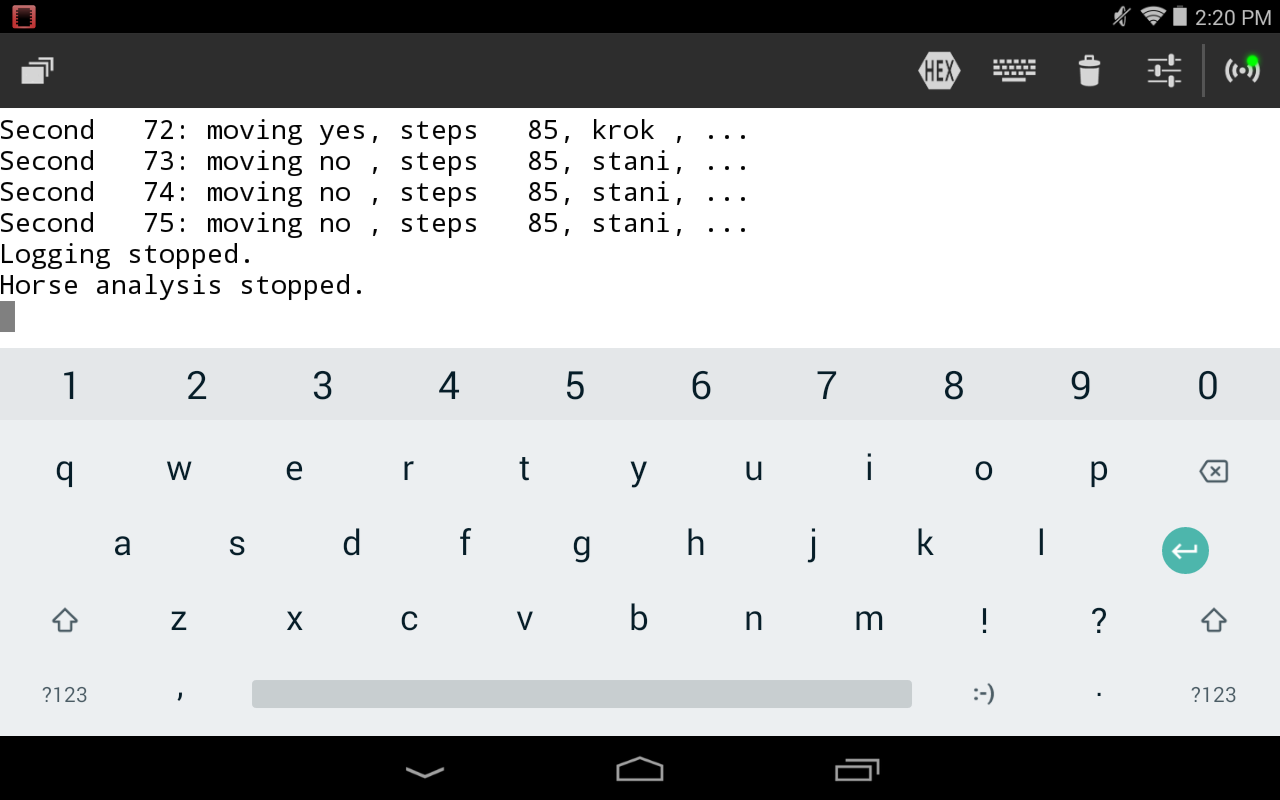
\includegraphics[width=\linewidth]{img/HorseAnalysisTablet.png}
\end{figure}

This tool demonstrates that the \ind{SensorBoard} is able to run some user code in real-time with real-time results.

\subsection{Controlling via \ac{TCP}}
The application can be controlled via \ac{TCP} connection using single letter commands. I recommend implementing a web-page based user interface in the future versions of the application. One letter commands are used because it is the easiest way how to control the board from a tablet with on-screen keyboard only. I would recommend using the more advanced protocol in the future versions. All the communication is possible via \ac{TCP} connection or UART through USB connection. The control commands are:

\begin{itemize}
    \item[\textbf{r}] Reset the board and restart the application. We get the same result when we switch the board off and on.
    \item[\textbf{p}] Ping command. When received, the text "Ping received." is printed.
    \item[\textbf{h}] Start/stop the horse movement analysis. When the analysis is running the text output is sent every second.
    \item[\textbf{s}] Start/stop streaming the raw data from the sensors.
    \item[\textbf{l}] Start/stop logging the raw data from the sensors to the SD card. When the logging is in progress, the green software LED is ON on the \ind{SensorBoard}.
\end{itemize}

\subsection{Using multiple SensorBoards}
When we have more \ind{SensorBoard}s, we can connect them like in figure \ref{UELogging2}. Then all the hardware connected together behaves like one \ind{SensorBoard} with so many sensors in different places. All the \ind{SensorBoard}s should connect to one WiFi network created by one board or by an external WiFi access point (e.g., mobile phone hotspot). All the \ind{SensorBoard}s except one (configured on SD card) behaves as \ac{TCP} clients and connects to \ac{TCP} server (the last \ind{SensorBoard}). The \ac{TCP} server resends all the commands to the other boards, so all the \ind{SensorBoard}s behaves synchronously. The log files are stored on the SD card inside each device and the names of these files are the same on all connected boards. So, the \ac{TCP} server dictates the names of all log files. One synchronous session creates multiple files on multiple SD cards, but with the same filenames on all devices. The whole system of connected boards can be used like in figure \ref{UELoggingHorse}.
